% This must be in the first 5 lines to tell arXiv to use pdfLaTeX, which is strongly recommended.
\pdfoutput=1
% In particular, the hyperref package requires pdfLaTeX in order to break URLs across lines.

\documentclass[11pt]{article}

% Change "review" to "final" to generate the final (sometimes called camera-ready) version.
% Change to "preprint" to generate a non-anonymous version with page numbers.
\usepackage[final]{acl}

% Standard package includes
\usepackage{times}
\usepackage{latexsym}

% For proper rendering and hyphenation of words containing Latin characters (including in bib files)
\usepackage[T1]{fontenc}
% For Vietnamese characters
% \usepackage[T5]{fontenc}
% See https://www.latex-project.org/help/documentation/encguide.pdf for other character sets

% This assumes your files are encoded as UTF8
\usepackage[utf8]{inputenc}

% This is not strictly necessary, and may be commented out,
% but it will improve the layout of the manuscript,
% and will typically save some space.
\usepackage{microtype}

% This is also not strictly necessary, and may be commented out.
% However, it will improve the aesthetics of text in
% the typewriter font.
\usepackage{inconsolata}

%Including images in your LaTeX document requires adding
%additional package(s)
\usepackage{graphicx}

\usepackage{longtable}
\usepackage{enumitem}
\usepackage{array}
\newcommand{\todo}[1]{\color{red}#1\color{black}}

% If the title and author information does not fit in the area allocated, uncomment the following
%
%\setlength\titlebox{<dim>}
%
% and set <dim> to something 5cm or larger.

\title{Goldfish: Monolingual Language Models for 350 Languages}

% Author information can be set in various styles:
% For several authors from the same institution:
% \author{Author 1 \and ... \and Author n \\
%         Address line \\ ... \\ Address line}
% if the names do not fit well on one line use
%         Author 1 \\ {\bf Author 2} \\ ... \\ {\bf Author n} \\
% For authors from different institutions:
% \author{Author 1 \\ Address line \\  ... \\ Address line
%         \And  ... \And
%         Author n \\ Address line \\ ... \\ Address line}
% To start a separate ``row'' of authors use \AND, as in
% \author{Author 1 \\ Address line \\  ... \\ Address line
%         \AND
%         Author 2 \\ Address line \\ ... \\ Address line \And
%         Author 3 \\ Address line \\ ... \\ Address line}

\author{Tyler A. Chang$^{1,2}$, \quad Catherine Arnett$^3$, \quad Zhuowen Tu$^1$, \quad Benjamin K. Bergen$^1$ \\
$^1$Department of Cognitive Science \\
$^2${Halıcıoğlu} Data Science Institute \\
$^3$Department of Linguistics \\
University of California San Diego \\
{\texttt{$\{$tachang, ccarnett, ztu, bkbergen$\}$@ucsd.edu}}
}

\begin{document}
\maketitle
\begin{abstract}
For many low-resource languages, the only available language models are large multilingual models trained on many languages simultaneously.
However, using FLORES perplexity as a metric, we find that these models perform worse than bigrams for many languages (e.g. 24\% of languages in XGLM 4.5B; 43\% in BLOOM 7.1B).
To facilitate research that focuses on low-resource languages, we pre-train and release Goldfish, a suite of monolingual autoregressive Transformer language models up to 125M parameters for 350 languages.
The Goldfish reach lower FLORES perplexities than BLOOM, XGLM, and \mbox{MaLA-500} on 98 of 204 FLORES languages, despite each Goldfish model being over 10$\times$ smaller.
However, the Goldfish significantly underperform larger multilingual models on reasoning benchmarks, suggesting that for low-resource languages, multilinguality primarily improves general reasoning abilities rather than basic text generation.
We release models trained on 5MB (350 languages), 10MB (288 languages), 100MB (166 languages), and 1GB (83 languages) of text data where available.
The Goldfish models are available as baselines, fine-tuning sources, or augmentations to existing models in low-resource NLP research, and they are further useful for crosslinguistic studies requiring maximally comparable models across languages.
\end{abstract}

\section{Introduction}
Language modeling research in low-resource languages often relies on large multilingual models trained on many languages simultaneously \citep{conneau-etal-2020-unsupervised,adelani-etal-2021-masakhaner,ebrahimi2021americasnli,lin2022xglm,hangya2022improving,imanigooghari-etal-2023-glot500}.
For many low-resource languages, a dedicated model optimized for that language does not exist.
This lack of dedicated models hinders comparability of results across models and languages \citep{bandarkar2024belebele}, and it contributes to model under-performance in low-resource languages \citep{wu-dredze-2020-languages,blasi2022systematic}.
These barriers to research in low-resource languages are likely to exacerbate existing inequities across language communities in NLP research \citep{bender2011achieving,joshi-etal-2020-state}.

To address this lack of available models, we introduce Goldfish, a suite of over 1000 monolingual language models for 350 diverse languages.\footnote{The name refers to shared qualities between our models and goldfish (\textit{Carassius auratus}); they are small, there are many of them, and they are known for their poor memories (perhaps inaccurately; \citealp{carey-2024-goldfish}).
% If an acronym is desired, Goldfish can stand for \textbf{G}enerative aut\textbf{O}regressive \textbf{L}ow-resource mo\textbf{D}els \textbf{F}or l\textbf{I}mited-compute \textbf{S}ystem \textbf{H}ardware.
}
The models reach lower perplexities than XGLM \citep{lin2022xglm}, BLOOM 7.1B \citep{bigscience-bloom}, and MaLA-500 \citep{lin-2024-mala500} on 98 out of 204 FLORES languages, despite each Goldfish model being over 10$\times$ smaller.
The Goldfish also outperform simple bigram models, which are surprisingly competitive with larger models for low-resource languages (e.g. lower perplexities than BLOOM 7.1B on 43\% of its languages; \S\ref{sec:flores-ppls}).
However, despite better perplexities, the Goldfish underperform larger multilingual models on reasoning benchmarks, suggesting that multilingual pre-training may benefit abstract reasoning capabilities over more basic grammatical text generation (\S\ref{sec:reasoning}).

\setlength{\belowcaptionskip}{-0.3cm}
% \setlength\tabcolsep{3pt}
\begin{figure*}[t]
    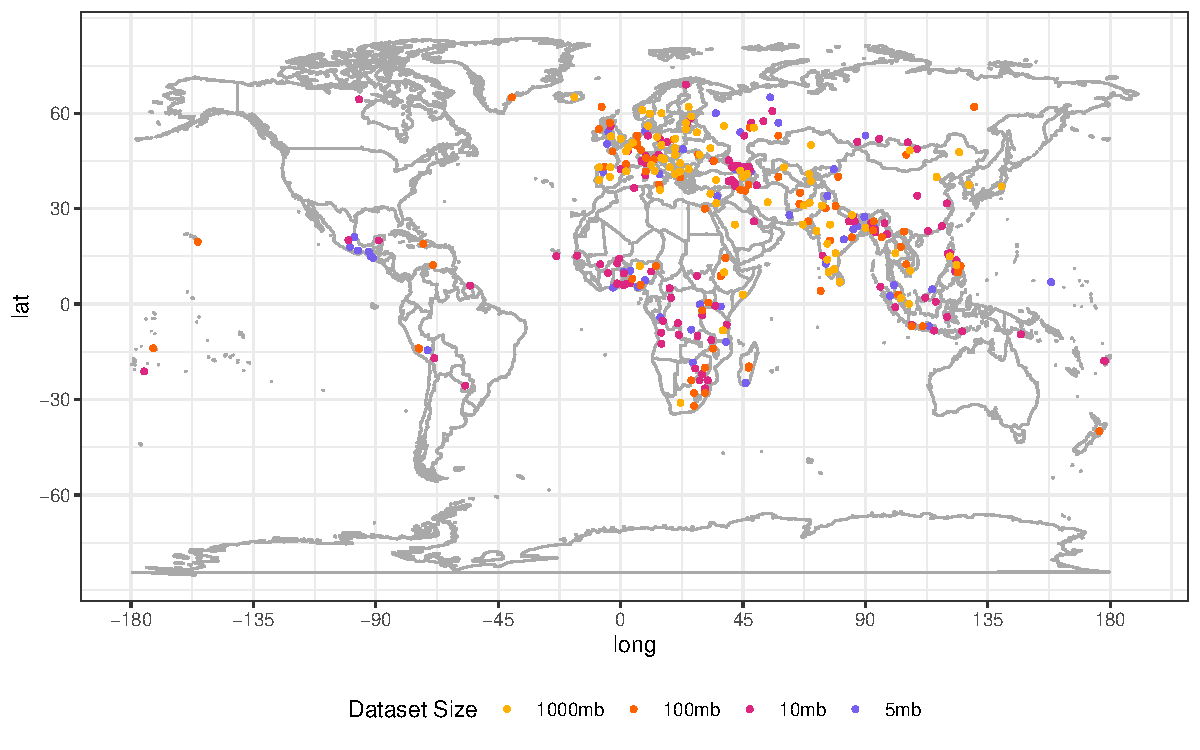
\includegraphics[width=7.5cm,trim={0 1.5cm 0 0},clip]{figures/goldfish_map.pdf} \hspace{0.0cm}
    \raisebox{2.1cm}{
    \footnotesize
    \definecolor{fish5}{HTML}{785EF0}
    \definecolor{fish10}{HTML}{DC267F}
    \definecolor{fish100}{HTML}{FE6100}
    \definecolor{fish1000}{HTML}{FFB000}
    \renewcommand{\arraystretch}{1.3}
    \begin{tabular}{| >\raggedleft p{1.2cm}| >{\raggedright\arraybackslash} p{5.5cm}|}
        \hline
        Data size & Model output \\
        \hline
        \textcolor{fish5}{\textbf{5MB}} & \texttt{``Goldfish are \color{fish5} a few years of the most of the most of the most\color{black}...''} \\
        \textcolor{fish10}{\textbf{10MB}} & \texttt{``Goldfish are \color{fish10} a great way to the best way to the best way\color{black}...''} \\
        \textcolor{fish100}{\textbf{100MB}} & \texttt{``Goldfish are \color{fish100} a great way to get your fish in the wild.\color{black}''} \\
        \textcolor{fish1000}{\textbf{1GB}} & \texttt{``Goldfish are \color{fish1000} a species of fish that are found in the sea.\color{black}''} \\
        \hline
    \end{tabular}}
    \normalsize
    \caption{Left: Map of the 350 languages for which Goldfish models are available, using coordinates from Glottolog \citep{hammarstrom-etal-2021-glottolog}. Right: Sample model outputs completing the prompt \texttt{``Goldfish are''} for the \texttt{eng\_latn} (English) model for each dataset size, using sampling temperature zero. Grammatical text generation begins to emerge in the 100MB-dataset model (available for 166 languages), but the lower-resource models still achieve better perplexities than previous models for many low-resource languages (\S\ref{sec:flores-ppls}).
    }
    \label{fig:map-outputs}
\end{figure*}
\setlength{\belowcaptionskip}{0cm}

Finally, to enable comparisons across languages, we release monolingual models trained on comparable dataset sizes for all languages: 5MB, 10MB, 100MB, and 1GB when available, after accounting for the fact that languages require different numbers of UTF-8 bytes to encode comparable content (\citealp{arnett2024bit}).
These Goldfish serve as baselines, allowing results in diverse languages to be situated relative to comparable models.
They can also be used as source models for fine-tuning or to enhance larger multilingual models in areas where those models fall short (\S\ref{sec:flores-ppls}).
Models and code are available at \url{https://huggingface.co/goldfish-models}.


\section{Related Work}
Low resource language modeling often leverages multilingual pre-training, where a model is trained on multiple languages simultaneously \citep{pires2019multilingual,conneau-etal-2020-unsupervised}.
Indeed, this can improve low-resource performance, particularly when models have sufficient capacity and the multilingual data is from related or typologically similar languages \citep{kakwani2020indicnlpsuite,ogueji2021small,chang-etal-2023-multilinguality}.
However, monolingual models have still been shown to achieve better performance than multilingual models for many languages (e.g. \citealp{martin-etal-2020-camembert,pyysalo-etal-2021-wikibert,gutierrez2021maria,luukkonen-etal-2023-fingpt}).
Thus, it appears that existing multilingual language models are still limited by model capacity or limited data in low-resource languages \citep{conneau-etal-2020-unsupervised,chang-etal-2023-multilinguality}.

Notably, the training datasets for massively multilingual models are often heavily skewed towards high-resource languages.
For example, XGLM 4.5B is trained on over 7000$\times$ more Norwegian (71GB; 5.4M native speakers) than Quechua (0.01GB; 7.3M native speakers; \citealp{lin2022xglm,ethnologue-2024}).
In a more extreme case, BLOOM is trained on only 0.07MB of Akan (8.1M native speakers) out of 1.61TB total (\mbox{4e-6}\% of the pre-training dataset; \citealp{bigscience-bloom}).
These extremely small quantities of low-resource language data often do not leverage recent efforts to compile text data in low-resource languages \citep{costa2022no,imanigooghari-etal-2023-glot500,kudugunta-etal-2023-madlad400}, and the data imbalances are likely to severely hinder performance in low-resource languages.
Indeed, we find that these models have worse perplexities than simple bigram models for many languages (\S\ref{sec:flores-ppls}).
Unfortunately, comparable monolingual language models across many diverse languages have yet to be studied or released.

\section{Models and Datasets}
We introduce the Goldfish models, a suite of 1154 monolingual Transformer language models pre-trained for 350 languages. The largest model for each language is 125M parameters.
We train models on 5MB, 10MB, 100MB, and 1GB of text when available after byte premium scaling \citep{arnett2024bit}.
Figure \ref{fig:map-outputs} shows a geographic map of the 350 languages, with coordinates from Glottolog \citep{hammarstrom-etal-2021-glottolog}, along with sample outputs from the English model for each dataset size.

\setlength{\belowcaptionskip}{-0.35cm}
% \setlength\tabcolsep{3pt}
\begin{table*}[t]
    \centering
    \footnotesize
    \renewcommand{\arraystretch}{1.3}
    \begin{tabular}{|p{2.4cm}|c|cccc|}
        \cline{1-6}
        Goldfish data size &
        \multicolumn{1}{c|}{\# Langs} &
        \multicolumn{1}{c|}{Goldfish} &
        \multicolumn{1}{c|}{Bigrams} &
        \multicolumn{1}{c|}{XGLM 4.5B} &
        \multicolumn{1}{c|}{MaLA-500 10B} \\ 
        \hline
        1000MB & 73 & \textbf{76.9} & 112.3 & 78.6 & 84.7 \\
        100MB & 22 & \textbf{102.7} & 132.6 & 143.9 & 121.7 \\
        10MB, 5MB & 5 & \textbf{130.5} & 148.3 & 183.1 & 135.0 \\
        \hline
    \end{tabular}
    \normalsize
    \caption{Mean FLORES log-perplexity ($\downarrow$) for the 100 languages in XGLM 4.5B, MaLA-500, and FLORES, separated by maximum Goldfish dataset size. The Goldfish languages are a strict superset of these languages.
    }
    \label{tab:mean-ppls}
\end{table*}
\setlength{\belowcaptionskip}{0cm}

\subsection{Training Datasets}
\label{sec:datasets}
We merge the massively multilingual text datasets compiled in \citet{chang-etal-2023-multilinguality}, Glot500 \citep{imanigooghari-etal-2023-glot500}, and MADLAD-400 (\citealp{kudugunta-etal-2023-madlad400}) per language.
To facilitate fair evaluations, we hold out FLORES-200 and AmericasNLI from all datasets \citep{costa2022no,ebrahimi2021americasnli}.
We deduplicate repeated sequences of 100 UTF-8 bytes and drop languages with only Bible data.
Full dataset details are in \S\ref{app:dataset-details}.

To sample pre-training datasets of the desired sizes in a language $L$, we first use the Byte Premium Tool \citep{arnett2024bit} to estimate the \textbf{byte premium} for $L$, the number of UTF-8 bytes required to encode comparable text in $L$ relative to \texttt{eng\_latn} (English).
For example, \texttt{khm\_khmr} (Khmer) has byte premium 3.91, meaning that it uses approximately 3.91$\times$ as many UTF-8 bytes as English to encode content-matched text.
We divide each dataset size by the estimated byte premium for the corresponding language, thus measuring all datasets in units of ``equivalent'' English text bytes.
We sample datasets to train monolingual language models on \textbf{5MB} (350 languages), \textbf{10MB} (288 languages), \textbf{100MB} (166 languages), and \textbf{1GB} (83 languages) when available after byte premium scaling.\footnote{The languages with 5MB-dataset models are a subset of the languages with 10MB-dataset models, and similarly for the 100MB and 1GB dataset sizes.}
These are equivalent to roughly 1M, 2M, 20M, and 200M tokens of English text respectively; including 10 epochs of repetition, the 1GB-dataset models are trained on the equivalent of roughly 2B English tokens.
When a 1GB dataset is not available for a language after byte premium scaling, we include a \textbf{full} model (267 languages) trained on the entire dataset in that language, for use cases that seek to maximize performance in a specific low-resource language.

\subsection{Architectures and Pre-Training}
\label{sec:model-training}

For each language and each dataset size, we pre-train an autoregressive GPT-2 Transformer language model from scratch \citep{radford-etal-2019-language}.
For the 1GB, 100MB, and full dataset sizes, we use the 125M-parameter architecture equivalent to GPT-1 \citep{radford-etal-2018-improving}, which has a similar parameter count to BERT-base and RoBERTa \citep{devlin-etal-2019-bert,liu-etal-2019-roberta}.
Because larger models do not appear to outperform smaller models for very small datasets \citep{chang-etal-2023-multilinguality}, we use the small model size (39M parameters) from \citet{turc2019well} for the 10MB and 5MB dataset sizes.
Full hyperparameters are reported in \S\ref{app:pretraining-details}.

We tokenize each dataset using using a monolingual SentencePiece tokenizer \citep{kudo-richardson-2018-sentencepiece} trained on that dataset size, limiting tokenizer training text to 100MB after byte premium scaling.
Following \citet{liu-etal-2019-roberta}, we use vocabulary size 50K and a maximum sequence length of 512 tokens for all models.
We train each language model on 10 epochs of its corresponding dataset.\footnote{Multiple epochs of pre-training is beneficial in data-constrained scenarios \citep{muennighoff-etal-2023-scaling}, but we find that more than 10 epochs of training leads to overfitting for extremely small datasets (e.g. 5MB).}
Pre-training details, compute costs, and all available models are reported in \S\ref{app:pretraining-details}.

\setlength{\belowcaptionskip}{-0.1cm}
% \setlength\tabcolsep{3pt}
\begin{table*}[t]
    \centering
    \footnotesize
    \renewcommand{\arraystretch}{1.3}
    \begin{tabular}{|p{2.0cm}|ccccc|}
        \cline{2-6}
        \multicolumn{1}{c|}{} &
        \multicolumn{1}{c|}{Bigrams} &
        \multicolumn{1}{c|}{XGLM 4.5B} &
        \multicolumn{1}{c|}{XGLM 7.5B} &
        \multicolumn{1}{c|}{BLOOM 7.1B} &
        \multicolumn{1}{c|}{MaLA-500 10B} \\ 
        \hline
        Bigrams & & 24 / 102 & 0 / 30 & 20 / 46 & 11 / 175 \\
        Goldfish (ours) & \textbf{202} / 202 & \textbf{60} / 102 & 2 / 30 & \textbf{32} / 46 & \textbf{111} / 175 \\
        \hline
    \end{tabular}
    \normalsize
    \caption{FLORES perplexity win rates for each row vs. column model. For example, Goldfish reach lower log-perplexities than MaLA-500 for 111/175 (63\%) of FLORES languages in both Goldfish and MaLA-500.}
    \label{tab:win-rates}
\end{table*}
\setlength{\belowcaptionskip}{0cm}

\setlength{\belowcaptionskip}{-0.3cm}
% \setlength\tabcolsep{3pt}
\begin{table*}[t]
    \centering
    \footnotesize
    \renewcommand{\arraystretch}{1.3}
    \begin{tabular}{|p{1.9cm}|c|cccccc|}
        \cline{2-8}
        \multicolumn{1}{c|}{} &
        \multicolumn{1}{c|}{\# Langs} &
        \multicolumn{1}{c|}{Chance} &
        \multicolumn{1}{c|}{Goldfish} &
        \multicolumn{1}{c|}{XGLM 4.5B} &
        \multicolumn{1}{c|}{XGLM 7.5B} &
        \multicolumn{1}{c|}{BLOOM 7.1B} &
        \multicolumn{1}{c|}{MaLA-500 10B} \\ 
        \hline
        Belebele & 121 & 25.0 & 28.2 & 30.1 & \textbf{30.6} & 30.2 & \textbf{30.6} \\
        XCOPA & 11 & 50.0 & 54.9 & 57.9 & \textbf{60.6} & 56.9 & 55.6 \\
        XStoryCloze & 10 & 50.0 & 52.5 & 57.1 & \textbf{59.9} & 58.2 & 55.7 \\
        \hline
    \end{tabular}
    \normalsize
    \caption{Reasoning benchmark accuracies averaged over non-English languages.
    Despite better perplexities, the Goldfish perform significantly worse than larger multilingual models on reasoning.
    }
    \label{tab:reasoning-results}
\end{table*}
\setlength{\belowcaptionskip}{0cm}

\section{FLORES Log-Perplexity Evaluations}
\label{sec:flores-ppls}
We first evaluate our models on FLORES-200 log-perplexity \citep{costa2022no} (equivalently, negative log-likelihood; \citealp{lin-2024-mala500}).
To avoid tokenization confounds from computing log-perplexity per token, we compute log-perplexity per FLORES sequence.
Regardless of its tokenization, a language model $\mathcal{M}$ assigns some probability $P_{\mathcal{M}}(s)$ to each sequence $s$ in FLORES.
In most cases, $s$ is a single sentence.
For fair comparison with multilingual models that need to determine the input language during the early parts of a sequence, we compute log-perplexity of the second half $s_1$ of each sequence given the first half $s_0$.
We then compute the mean over sequences:
\setlength{\abovedisplayskip}{0.2cm}
\setlength{\belowdisplayskip}{0.2cm}
\begin{equation}
\label{eq:ppl}
\textrm{LogPPL}_{\mathcal{M}} = \textrm{mean}_{s} \Big( - \textrm{log}( P_{\mathcal{M}}(s_1 | s_0)) \Big)
\end{equation}
A lower log-perplexity indicates better performance, where $\mathcal{M}$ assigns higher probabilities to ground truth text (FLORES sequences).
While imperfect, perplexity does not require annotated text data, it is predictive of performance on a variety of downstream tasks 
\citep{xia-etal-2023-training}, and it has been used to measure language model quality in previous work \citep{kaplan-etal-2020-scaling,hoffmann-etal-2022-training,lin-2024-mala500}.

We compare the Goldfish models with XGLM 4.5B (\citealp{lin2022xglm}; 134 languages), XGLM 7.5B (30 languages), BLOOM 7.1B (\citealp{bigscience-bloom}; 46 languages), and MaLA-500 10B (\citealp{lin-2024-mala500}; 534 languages).
We also compare to simple bigram models trained on the Goldfish datasets.\footnote{Bigram and perplexity implementation details in \S\ref{app:flores-details}.}
In all cases, we use the Goldfish model trained on the maximum amount of data in each language (maximum 1GB).

\paragraph{FLORES log-perplexity results.}
The Goldfish reach lower log-perplexities than all four comparison models on 98 of the 204 FLORES languages.
Average log-perplexities for the 100 FLORES languages included in both XGLM 4.5B and MaLA-500 are reported in Table~\ref{tab:mean-ppls} (excluding XGLM 7.5B and BLOOM 7.1B there because they are trained on far fewer languages).
On average, the Goldfish reach 13\% lower log-perplexities than XGLM 4.5B, and 11\% lower than MaLA-500 10B.

To ensure that these results are not driven by a small subset of specific languages, in Table~\ref{tab:win-rates} we report the pairwise ``win'' rates for Goldfish and bigrams vs. all four comparison models, for the set of FLORES languages shared between each pair.
The Goldfish models have a perplexity win rate above 50\% against all comparison models except XGLM 7.5B, which considers only 30 fairly high-resource languages \citep{lin2022xglm}.
Notably, the bigram models also reach lower perplexities than large multilingual models for a nontrivial number of languages: 24\% of languages in XGLM 4.5B and 43\% of languages in BLOOM 7.1B.
Still, the bigrams have worse perplexities than Goldfish for all languages.
Log-perplexities for individual languages and models are reported in Table~\ref{tab:ppl-table}.



\section{Multilingual Reasoning Benchmarks}
\label{sec:reasoning}
Because FLORES perplexities are not necessarily reflective of complex capabilities in language models, we also evaluate Goldfish, XGLM, BLOOM, and MaLA-500 (as in \S\ref{sec:flores-ppls}) on non-English Belebele (121 languages, reading comprehension; \citealp{bandarkar2024belebele}), XCOPA (11 languages, commonsense; 
\citealp{ponti-etal-2020-xcopa}), and XStoryCloze (10 languages, story commonsense; \citealp{lin2022xglm}).
All models are evaluated zero shot with no fine-tuning.
Evaluation task details are in \S\ref{app:reasoning-tasks}.

Results for all three reasoning tasks are reported in Table~\ref{tab:reasoning-results}.
Although all models perform quite poorly (close to chance accuracy), the Goldfish perform substantially worse than the multilingual models.\footnote{It is unlikely that this effect is due to model size alone; the Goldfish models (125M parameters) have easily enough capacity for their maximum of 1GB of text data.}
This indicates that the combination of larger datasets and model sizes in multilingual pre-training can allow language models to develop reasoning capabilities in specific languages, even when perplexities in those languages remain high.
For example, XGLM 7.5B has worse perplexities than Goldfish for 82 Belebele languages (in fact, worse than bigrams for 77 languages), but it outperforms Goldfish on Belebele (reading comprehension) for 56 of those languages.
This is in stark contrast with monolingual language models, which generally must reach low perplexities and acquire basic grammatical capabilities before developing reasoning abilities \citep{liu-etal-2021-probing-across,choshen-etal-2022-grammar,xia-etal-2023-training,chang2024characterizinglearningcurveslanguage}.
Intuitively, it may be that abstract reasoning patterns are often more language-agnostic than grammatical text generation, and thus multilingual pre-training primarily benefits the former.

\section{Conclusion}
We pre-train and release Goldfish, a suite of over 1000 monolingual language models for 350 languages.
The Goldfish achieve perplexities that are competitive with, and on average lower than, state-of-the-art multilingual language models across languages.
However, they underperform large multilingual models on reasoning tasks; in low-resource languages, it appears that multilingual pre-training facilitates nontrivial reasoning capabilities despite extremely poor perplexities.
We publicly release all Goldfish models to be used as comparable baselines, fine-tuning sources, or augmentations to larger models (e.g. cross-lingual experts; \citealp{blevins2024breakingcursemultilingualitycrosslingual}) in future low-resource NLP research.

\section*{Limitations}

\paragraph{Comparability and availability.}
In order to include as many low-resource languages as possible, the Goldfish models are trained on corpora compiled from a wide variety sources (\S\ref{app:dataset-details}).
Still, 5MB of text (roughly 1M tokens) is not publicly available for many of the world's languages.
Even where text is available, corpora for different languages vary significantly both in cleanliness and domain coverage (e.g. news vs. social media vs. books).
Thus, while we release models trained on comparable quantities of text in different languages (including accounting for byte premiums; \citealp{arnett2024bit}; \S\ref{sec:datasets}), the models are not perfectly comparable across languages.
In fact, it is likely that such perfect comparability is impossible given the diversity of the world's languages, cultures, and language use.
Even directly translated datasets are not perfectly comparable across languages \citep{untranslatability}.
Thus, the Goldfish models aim to maximize model and dataset comparability across languages while still covering a wide variety of languages.

\paragraph{Monolinguality.}
By design, all of the Goldfish models are monolingual.
For low-resource languages, training on closely related languages would likely improve performance \citep{conneau-etal-2020-unsupervised,chang-etal-2023-multilinguality}.
However, adding multilingual data introduces concerns such as the choice of added languages (some languages have more closely related languages in our dataset than others), quantities of added data, and model capacity limitations.
To maximize comparability across languages and to allow the models to serve as clearly-defined baselines, we train all Goldfish models monolingually.
Of course, language-annotated text datasets inevitably contain mislabeled text, particularly for similar languages \citep{caswell-etal-2020-language,blevins-zettlemoyer-2022-language,kreutzer-etal-2022-quality}.
Thus, we cannot guarantee that our models are entirely free from cross-language contamination, although they are monolingual to the best ability of current language identification models.

\paragraph{Model and dataset sizes.}
Because the Goldfish are focused on low-resource languages, we restrict all models to 1GB of training text (after byte premium scaling; \citealp{arnett2024bit}).
For the majority of the world's languages, 1GB is sufficient to include all publicly available text data in the language.
At these small dataset sizes, larger models do not appear to provide significant benefit over smaller models \citep{kaplan-etal-2020-scaling,hoffmann-etal-2022-training,chang-etal-2023-multilinguality}.
Thus, the largest Goldfish model that we train for each language has 125M parameters and is trained on a maximum of 1GB of text.
This is the same model size as GPT-1 \citep{radford-etal-2018-improving} or BERT \citep{devlin-etal-2019-bert}, and the 1GB dataset size is approximately 20\% of the dataset size of GPT-1 \citep{radford-etal-2018-improving}.

\paragraph{Downstream tasks.}
We evaluate the Goldfish models on FLORES log-perplexity (\S\ref{sec:flores-ppls}) and three reasoning benchmarks (\S\ref{sec:reasoning}).
These are some of the only evaluations that can be used for autoregressive language models in many languages, but they have significant limitations.
Perplexity is not necessarily predictive of grammatical text generation \citep{hu-etal-2020-systematic} or complex reasoning capabilities \citep{levy2024tasktokensimpactinput}, but it still provides reasonable signal for model performance \citep{xia-etal-2023-training} and it is often used to roughly quantify language model quality \citep{kaplan-etal-2020-scaling,hoffmann-etal-2022-training}.
On the other hand, reasoning benchmarks require annotated datasets and thus often cover fewer languages.
One notable exception is Belebele (121 non-English languages; \citealp{bandarkar2024belebele}), but even large state-of-the-art models perform quite poorly on Belebele without tuning or few-shot prompting (\S\ref{sec:reasoning}).
Thus, our evaluations of model reasoning are not entirely conclusive; we may primarily be measuring heuristics that allow the models to perform only somewhat above chance (arguably, this might still be considered a basic form of ``reasoning'').
We hope that tractable evaluation datasets with broad language coverage will become increasingly available in the future.

\paragraph{Risks and dataset licensing.}
Trained on a maximum of 1GB of text each, the Goldfish models have very limited capabilities relative to modern language models in high-resource languages.
The Goldfish are trained on publicly-released corpora used in previous NLP research (\S\ref{app:dataset-details}), but we cannot guarantee that the data is free from offensive content or personally identifying information.
We do not redistribute the data itself.
Furthermore, our models are small, which reduces the likelihood that they will regurgitate memorized text \citep{carlini2023quantifyingmemorizationneurallanguage}.
As far as we are aware, we do not include any datasets that prohibit use for language model training.
We report all included datasets in \S\ref{app:dataset-details}.
We will remove models for affected languages if contacted by dataset owners.

\section*{Acknowledgments}
We would like to thank the UCSD Language and Cognition Lab for valuable discussion.
Some models were trained on hardware provided by the NVIDIA Corporation as part of an NVIDIA Academic Hardware Grant.
Some models were also trained on the UCSD Social Sciences Research and Development Environment (SSRDE). 
Zhuowen Tu is supported by NSF IIS-2127544.
Tyler Chang is partially supported by the UCSD HDSI graduate fellowship.

% Bibliography entries for the entire Anthology, followed by custom entries
%\bibliography{anthology,custom}
% Custom bibliography entries only
\bibliography{goldfish}

\appendix

\section{Appendix}
\label{sec:appendix}

\subsection{Training Dataset Details}
\label{app:dataset-details}

\paragraph{Data sources.}
As described in \S\ref{sec:datasets}, we merge the text datasets compiled in \citet{chang-etal-2023-multilinguality}, Glot500 \citep{imanigooghari-etal-2023-glot500}, and MADLAD-400 (clean split; \citealp{kudugunta-etal-2023-madlad400}).
These datasets include popular multilingual corpora such as OSCAR \citep{suarez2019asynchronous,AbadjiOrtizSuarezRomaryetal.2021}, Wikipedia \citep{wikipedia}, No Language Left Behind \citep{costa2022no}, and others.
Together, these datasets take advantage of both automatically crawled datasets with automated language identification and targeted datasets manually annotated for specific low-resource languages.
All included datasets are publicly available; see Limitations for licensing concerns.
Comprehensively, the Goldfish dataset includes:
\begin{itemize}[leftmargin=0.5cm,itemsep=0.1cm,topsep=0.25cm]
\item \citet{chang-etal-2023-multilinguality}:\newline
OSCAR \citep{suarez2019asynchronous,AbadjiOrtizSuarezRomaryetal.2021}, Wikipedia \citep{wikipedia}, No Language Left Behind \citep{costa2022no}, Leipzig Corpora Collection \citep{goldhahn2012building}, eBible translations \citep{eBible}, Tatoeba \citep{tiedemann2012parallel,tiedemann-2020-tatoeba}, AfriBERTa \citep{ogueji2021small},  NusaX \citep{winata2022nusax}, AmericasNLP \citep{mager2021findings}, Nunavut Hansard Inuktitut–English Parallel Corpus \citep{joanis2020inuktitut}, Cherokee-English ChrEn dataset \citep{zhang2020chren}, Cherokee Corpus \citep{cherokee_dict}, Cree Corpus \citep{teodorescu-etal-2022-cree}, Languages of Russia \citep{zaydelman2016}, Evenki Life newspaper \citep{zueva2020finite}, transcribed Fula Speech Corpora \citep{fula2023}, IsiXhosa \citep{isixhosa_ner_corpus}, Ewe Language Corpus \citep{gelr2021}, Makerere Luganda Corpora \citep{mukiibi2022makerere}, CMU Haitian Creole dataset \citep{haitian_cmu}, Tigrinya Language Modeling Dataset \citep{gaim2021monolingual}, and Ulukau \citep{ulukau}.
\item Glot500 \citep{imanigooghari-etal-2023-glot500}:\newline
AI4Bharat \citep{AI4Bharat},
AI FOR THAI LotusCorpus \citep{aiforthai},
Arabic Dialects Dataset \citep{el-haj-etal-2018-arabic},
AfriBERTa \citep{ogueji2021small},
AfroMAFT \citep{adelani-etal-2022-thousand,xue-etal-2021-mt5},
Anuvaad \citep{Anuvaad},
AraBench \citep{sajjad-etal-2020-arabench},
Autshumato \citep{Autshumato}
Bloom Library \citep{DBLP:conf/emnlp/LeongNMFOW22}, 
CC100 \citep{conneau-etal-2020-unsupervised}, 
CCNet \citep{wenzek-etal-2020-ccnet}, 
CMU Haitian Creole \citep{haitian_cmu},
SADiLaR NCHLT corpus \citep{sadilar},
Clarin \citep{clarin},
DART \citep{alsarsour-etal-2018-dart},
Earthlings \citep{DBLP:journals/lre/Dunn20}, 
FFR Dataset \citep{ffr},
GiossaMedia \citep{gongora-etal-2022-use, gongora-etal-2021-experiments},
Glosses \citep{camacho-collados-etal-2016-large},
Habibi \citep{el-haj-2020-habibi},
HinDialect \citep{bafna2022empirical}, 
HornMT \citep{HornMT},
IITB \citep{kunchukuttan-etal-2018-iit},
IndicNLP \citep{nakazawa-etal-2021-overview},
Indiccorp \citep{kakwani2020indicnlpsuite}, 
isiZulu \citep{isizulu},
JParaCrawl \citep{morishita-etal-2020-jparacrawl}, 
kinyarwandaSMT \citep{KinyaSMT},
LeipzigData \citep{goldhahn2012building}, 
LINDAT \citep{lindat},
Lingala Song Lyrics \citep{lingala-songs},
LyricsTranslate \citep{lyrics-translate},
mC4 \citep{raffel-etal-2020-exploring}, 
MTData \citep{gowda-etal-2021-many}, 
MaCoCu \citep{DBLP:conf/eamt/BanonEFGKLNSRRS22}, 
Makerere MT Corpus \citep{mukiibi2022makerere},
Masakhane Community \citep{masakhane},
Mburisano Covid Corpus \citep{mburisano},
Menyo20K \citep{adelani-etal-2021-effect},
Minangkabau corpora \citep{koto-koto-2020-towards}, 
MoT \citep{palen-michel-etal-2022-multilingual},
NLLB seed \citep{costa2022no},
Nart Abkhaz text \citep{abkhaz},
OPUS \citep{tiedemann2012parallel}, 
OSCAR \citep{suarez2019asynchronous}, 
ParaCrawl \citep{banon-etal-2020-paracrawl},
Parallel Corpora for Ethiopian Languages \citep{teferra-abate-etal-2018-parallel}, 
Phontron \citep{neubig11kftt},
QADI \citep{abdelali-etal-2021-qadi},
Quechua-IIC \citep{zevallos2022introducing}, 
SLI GalWeb.1.0 \citep{agerri-etal-2018-developing},
Shami \citep{abu-kwaik-etal-2018-shami},
Stanford NLP \citep{stanford-nlp},
StatMT \citep{statmt},
TICO \citep{anastasopoulos-etal-2020-tico},
TIL \citep{mirzakhalov-etal-2021-large},
Tatoeba \citep{tiedemann-2020-tatoeba},
TeDDi \citep{moran-etal-2022-teddi},
Tilde \citep{rozis-skadins-2017-tilde},
W2C \citep{11858/00-097C-0000-0022-6133-9}, 
WAT \citep{nakazawa-etal-2022-overview},
WikiMatrix \citep{schwenk-etal-2021-wikimatrix}, 
Wikipedia \citep{wikipedia},
Workshop on NER for South and South East Asian Languages \citep{singh-2008-named}, and XLSum \citep{xlsum}.

\item MADLAD-400 \citep{kudugunta-etal-2023-madlad400}:\newline
CommonCrawl \citep{commoncrawl-2022}.
\end{itemize}
We start with the corpus from \citet{chang-etal-2023-multilinguality}.
We then merge the dataset per language with Glot500 for languages that have not yet reached our 1GB maximum (after byte premium scaling).
Then, we merge the dataset with MADLAD-400 for languages that have still not reached our 1GB maximum.
We also add MADLAD-400 for languages with short average line lengths (less than 25.0 tokens), to make use of MADLAD-400's longer contiguous sequences.
To allow comparisons on popular low-resource language evaluations, we exclude FLORES-200 \citep{costa2022no} and AmericasNLI \citep{ebrahimi2021americasnli} from all dataset merging.
For each dataset, we exclude languages that contain only Bible data.
Because there is likely significant overlap between different dataset sources, we deduplicate repeated sequences of 100 UTF-8 bytes for each language \citep{lee2021deduplicating}.

\paragraph{Language codes.}
To enable dataset merging per language, several datasets must be converted to ISO 639-3 language codes and ISO 15924 script codes.
In some cases, this introduces ambiguity because datasets can be labeled as individual language codes (e.g. \texttt{quy\_latn} for Ayacucho Quechua and \texttt{quz\_latn} for Cusco Quechua) or as macrolanguage codes (e.g. \texttt{que\_latn} for Quechua).
In these cases, we compile both a macrolanguage dataset and individual language datasets.
Datasets labeled with individual codes contribute both to their individual dataset and their umbrella macrolanguage dataset; datasets labeled with macrolanguage codes contribute only to the macrolanguage dataset.
For example, we have individual \texttt{quy\_latn} and \texttt{quz\_latn} datasets, both of which contribute to a larger \texttt{que\_latn} dataset, which also contains datasets labeled only with \texttt{que\_latn}.
These ambiguities primarily appear for lower-resource languages.

Additionally, we drop several redundant language codes:
\begin{itemize}[leftmargin=0.5cm,itemsep=0.0cm,topsep=0.1cm]
\item We drop \texttt{ory\_orya} (Odia) in favor of the macrocode \texttt{ori\_orya} because \texttt{ory\_orya} is the only individual language within \texttt{ori\_orya} for which we have any data.
\item For the same reason, we drop \texttt{npi\_deva} (Nepali) in favor of the macrocode \texttt{nep\_deva}.
\item For the same reason, we drop \texttt{swh\_latn} (Swahili) in favor of the macrocode \texttt{swa\_latn}.
\item We drop \texttt{cmn\_hans} (Mandarin) in favor of the macrocode \texttt{zho\_hans} (Chinese) because the \texttt{zho\_hans} data is almost entirely in Mandarin. While less specific, \texttt{zho\_hans} is commonly used by other datasets.
For other Chinese languages, see their individual codes (e.g. \texttt{yue\_hant} for Cantonese).
We note that the similar code \texttt{zho\_hant} (traditional characters) is not primarily Mandarin.
\item We drop \texttt{hbs\_cyrl} and \texttt{hbs\_latn} (Serbo-Croatian) because we have the individual languages Serbian (\texttt{srp\_cyrl} and \texttt{srp\_latn}), Croatian (\texttt{hrv\_latn}), and Bosnian (\texttt{bos\_cyrl} and \texttt{bos\_latn}).
\item We drop the deprecated code \texttt{ajp\_arab} (Levantine Arabic) in favor of \texttt{apc\_arab}.
\item We drop \texttt{ber\_latn} (Berber) because it is a collective code for distinct (and often not mutually intelligible) languages. We keep the constituent individual languages.
\item We drop \texttt{nah\_latn} (Nahuatl) because it is a collective code for distinct languages. We keep the constituent individual languages.
\end{itemize}
After merging, we have a dataset of 547GB of text covering 523 language-script combinations (486 unique language codes, 32 unique script codes).

\paragraph{Byte premiums.}
As described in \S\ref{sec:datasets}, we then scale our dataset sizes by estimated byte premiums \citep{arnett2024bit}.
A byte premium $b$ for a language $L$ indicates that content-matched (i.e. parallel) text in $L$ takes $b\times$ as many UTF-8 bytes to encode as English.
We use the Byte Premium Tool \citep{arnett2024bit} to compute or estimate the byte premium for all of our languages.
Byte premiums are pre-computed in the tool for high-resource languages.
For each novel low-resource language $L$, we use the tool (which uses a linear regression) to predict the byte premium for $L$ based on the character entropy for text in $L$ and the script type for $L$ (alphabet, abjad, abugida, or logography), as recommended for low-resource languages in \citet{arnett2024bit}.
Then, we have an estimated byte premium for every language in our dataset.
We clip each byte premium to a minimum of 0.70 and a maximum of 5.00; clipping occurs for only three languages (\texttt{lzh\_hant}, \texttt{wuu\_hani} $\to$ 0.70, \texttt{mya\_mymr} $\to$ 5.00).
As described in \S\ref{sec:datasets}, all of our training datasets (both for tokenizers and for the models themselves) are sampled based on size in bytes after byte premium scaling.
We drop languages with less than 5MB of text after byte premium scaling.

\paragraph{Dataset statistics.}
The resulting 350 Goldfish languages cover five continents, 28 top-level language families \citep{hammarstrom-etal-2021-glottolog}, and 32 scripts (writing systems).
All languages for which Goldfish models are available are listed in Table~\ref{tab:lang-list}.
We include the language name, ISO 639-3 language code, ISO 15924 script code, estimated byte premium, dataset size after byte premium scaling, dataset size in tokens, and proportion of the dataset from each of our four largest sources.
Raw dataset sizes before byte premium scaling can be obtained by multiplying the dataset size after byte premium scaling by the estimated byte premium.
Source dataset proportions are reported before deduplication.
The reported dataset sizes reflect the dataset for the Goldfish model trained on the maximum amount of data for that language (the \textbf{1GB}-dataset Goldfish when available, otherwise the \textbf{full}-dataset Goldfish).
Reported token counts use the tokenizer for the largest Goldfish model for that language.
All dataset statistics can be downloaded at \url{https://github.com/tylerachang/goldfish}.


\subsection{Pre-Training Details}
\label{app:pretraining-details}
As described in \S\ref{sec:model-training}, we train monolingual language models for five dataset sizes when available after byte premium scaling: \textbf{5MB}, \textbf{10MB}, \textbf{100MB}, \textbf{1GB}, and \textbf{full}.
The full dataset size (including all available data) is only included if a 1GB dataset is not available for a language.
In total, the Goldfish include 350 5MB-dataset models, 288 10MB-dataset models, 166 100MB-dataset models, 83 1GB-dataset models, and 267 full-dataset models (1154 models total).
Full hyperparameters are reported in Table \ref{tab:hyperparameters}.

\setlength\tabcolsep{3pt}
\begin{table}[t]
    \centering
    \small
    \renewcommand{\arraystretch}{1.11}
    \begin{tabular}{|>{\raggedright}p{3.2cm}|r|r|}
    \hline
    \textbf{Hyperparameter} & \textbf{5MB,10MB} & \textbf{100MB,1GB,full} \\
    \hline
    Total parameters & 39M & 125M \\
    Layers & 4 & 12 \\
    Embedding size & 512 & 768 \\
    Hidden size & 512 & 768 \\
    Intermediate hidden size & 2048 & 3072 \\
    Attention heads & 8 & 12 \\
    Attention head size & 64 & 64 \\
    \hline
    Learning rate & \multicolumn{2}{r|}{1e-4} \\
    Batch size & \multicolumn{2}{r|}{5MB: 4, 10MB: 8,} \\
    & \multicolumn{2}{r|}{100MB: 32, 1GB: 64} \\
    Epochs & \multicolumn{2}{r|}{10} \\
    Activation function & \multicolumn{2}{r|}{GELU} \\
    Max sequence length & \multicolumn{2}{r|}{512} \\
    Position embedding & \multicolumn{2}{r|}{Absolute} \\
    Learning rate decay & \multicolumn{2}{r|}{Linear} \\
    Warmup steps & \multicolumn{2}{r|}{10\% of pre-training} \\
    Adam $\epsilon$ & \multicolumn{2}{r|}{1e-6} \\
    Adam $\beta_1$ & \multicolumn{2}{r|}{0.9} \\
    Adam $\beta_2$ & \multicolumn{2}{r|}{0.999} \\
    Dropout & \multicolumn{2}{r|}{0.1} \\
    Attention dropout & \multicolumn{2}{r|}{0.1} \\
    \hline
    \end{tabular}
    \caption{Pre-training hyperparameters for Goldfish trained on different dataset sizes \citep{devlin-etal-2019-bert,turc2019well,radford-etal-2018-improving}.}
    \label{tab:hyperparameters}
\end{table}
% Vocab size varies slightly if tokenizer vocabulary is not filled.

\paragraph{Tokenizers.}
All tokenizers are trained with vocabulary size 50K \citep{liu-etal-2019-roberta} on the same dataset size as their corresponding model (including byte premium scaling).
We use SentencePiece tokenizers \citep{kudo-richardson-2018-sentencepiece} with training text randomly sampled from the dataset for the desired language.
To avoid memory errors, we limit tokenizer training text to 100MB after byte premium scaling.
After tokenizer training, we tokenize each training dataset, concatenating text lines such that each sequence contains exactly 512 tokens.
We run tokenization before shuffling and sampling to the desired dataset sizes, so our sequences of 512 tokens preserve contiguous text where possible, although several of our source corpora only exist in shuffled form.
Finally, we sample our tokenized datasets to 5MB, 10MB, 100MB, and 1GB after byte premium scaling.\footnote{When de-tokenized, the tokenized datasets result in slightly smaller datasets than the original text datasets, because the tokenizer truncates lines to create 512-token sequences. All reported dataset sizes account for this truncation.}

\paragraph{Architectures.}
All of our models use the GPT-2 architecture \citep{radford-etal-2019-language}, changing only the number of layers, attention heads, and embedding sizes as in \citet{turc2019well}.
For the 100MB-, 1GB-, and full-dataset models, we use the 125M-parameter architecture equivalent to GPT-1 \citep{radford-etal-2018-improving} (similar to BERT-base and RoBERTa; \citealp{devlin-etal-2019-bert,liu-etal-2019-roberta}).
Because smaller models perform similarly to larger models in low-resource scenarios \citep{chang-etal-2023-multilinguality}, we use the small model size (39M parameters) from \citet{turc2019well} for the 10MB and 5MB dataset sizes.

\paragraph{Training hyperparameters.}
Language models are pre-trained using the Hugging Face Transformers library \citep{wolf-etal-2020-transformers} and code from \citet{chang-bergen-2022-word}.
We refrain from extensive hyperparameter tuning to avoid biasing our hyperparameters towards English (or any other selected tuning language).
Instead, we adopt hyperparameters from previous work with minimal modifications.
To match the setup of our models and to prevent overfitting, we select hyperparameters based on models with fairly small training datasets relative to modern standards.
Specifically, following BERT \citep{devlin-etal-2019-bert}, we use learning rate 1e-4 for the 125M-parameter models (the same as RoBERTa for small batch sizes; \citealp{liu-etal-2019-roberta}; GPT-1 uses learning rate 2.5e-4; \citealp{radford-etal-2018-improving}).
Based on initial results using randomly-sampled languages, we find that learning rate 1e-4 also works well for the 39M-parameter models; this is in line with \citet{chang-etal-2023-multilinguality}, who find that learning rate 2e-4 works well for small models, and smaller learning rates reduce the speed of any potential overfitting.

We train each model for 10 epochs of the training data; multiple epochs of pre-training is beneficial in data-constrained scenarios \citep{muennighoff-etal-2023-scaling}, but pre-training on more than 10 epochs often leads to overfitting (increases in eval loss) in the 5MB scenarios.
For batch sizes, following GPT-1 (most similar to our models; \citealp{radford-etal-2018-improving}), we use batch size 64 (64$\times$512 = 32K tokens) for the 1GB-dataset models.
We find that these larger batch sizes lead to overfitting for small datasets, so we use batch sizes 4, 8, and 32 for \mbox{5MB-,} \mbox{10MB-,} and 100MB-dataset models respectively (determined based on initial experiments with randomly-sampled languages).
These correspond to batches of 2K, 4K, or 16K tokens.
For full-dataset models, we use the batch size that would be used if rounding the dataset size down to 5MB, 10MB, or 100MB (recall that we do not train a full-dataset model when the 1GB dataset is available for a language).

\paragraph{Compute costs.}
% 1.0586731489249398e+16 FLOPs.
All language model pre-training runs together take a total of $1.65 \times 10^{20}$ FLOPs.
This is less than $1/1900\times$ the computation used to train the original 175B-parameter GPT-3 model (\citealp{brown-etal-2020-language}; $3.14 \times 10^{23}$ FLOPs).
Models are each trained on one NVIDIA GeForce GTX TITAN X, GeForce RTX 2080 Ti, TITAN Xp, Quadro P6000, RTX A4500, RTX A5000, or RTX A6000 GPU.
% Approximately 15608.169958928287.
In total, Goldfish pre-training takes the equivalent of approximately 15600 A6000 GPU hours.
% 16 hours per larger model for FLORES, 48 hours for Belebele, others negligible.
Inference for FLORES perplexities and reasoning benchmarks takes approximately 250 A6000 GPU hours (primarily due to the large multilingual models used for comparison).
% CPU core hours: ~5 days * 8 cores (merging); ~7 days * 4 cores (tokenization).
% Total: (40 + 28) * 24 hours
Dataset merging, deduplication, and tokenization takes approximately 1600 CPU core hours.

\subsection{FLORES Evaluation Details}
\label{app:flores-details}

In \S\ref{sec:flores-ppls}, we evaluate the Goldfish models, XGLM 4.5B, XGLM 7.5B, BLOOM 7.1B, MaLA-500 10B, and bigram models on FLORES log-perplexity (negative log-likelihood).
For each FLORES sequence $s$, we compute the probability of the second half $s_1$ of the sequence given the first half $s_0$.
The first and second half are determined based on number of characters, so the halfway split is the same for all models considered.
We round to the nearest token when the halfway split is in the middle of a subword token.
Each model $\mathcal{M}$ then assigns some probability $P_{\mathcal{M}}(s_1 | s_0)$ regardless of tokenization, except for rounding the halfway point to the nearest token.
The probability for any [UNK] (unknown) token is set to random chance $1/v$ where $v$ is the tokenizer vocabulary size.\footnote{Otherwise, for unseen writing systems (e.g. Tibetan script \texttt{tibt} in XGLM), the probability $P(\textrm{[UNK]} | \textrm{[UNK] [UNK] ...})$ is very high, resulting in artificially low perplexities. Setting the [UNK] token probabilities to random chance has very little effect on log-perplexity scores except for the scenario of an unseen writing system.}
As our final log-perplexity score, we compute the mean negative-log-probability over all FLORES sequences in the target language.
Because perplexities generally use geometric means, we use arithmetic means for log-perplexities. 
The final equation is presented in Equation~\ref{eq:ppl}.

FLORES log-perplexities for all models and languages are reported in Table~\ref{tab:ppl-table}.
For Goldfish models, we report the log-perplexity for the model trained on the largest dataset for the language (i.e. the 1GB-dataset model when available, otherwise the full-dataset model).
Log-perplexities of the 5MB-, 10MB-, 100MB-, and 1GB-dataset models specifically are available at \url{https://github.com/tylerachang/goldfish}.

\paragraph{Bigram model details.}
For each FLORES language, we train a bigram model on the entire Goldfish dataset for that language, up to 1GB after byte premium scaling \S\ref{sec:datasets}.
The bigram model computes the probability of each token $w_i$ as $P(w_i | w_{i-1})$, computed based on raw bigram counts in the tokenized Goldfish dataset.
The tokenizer is the same as the Goldfish tokenizer for that dataset (i.e. the 1GB-dataset model when available, or the full-dataset model).
When a bigram is not observed in the dataset, we use backoff to unigram probability with a penalty multiplier of $\lambda=0.40$ (i.e. ``stupid backoff''; \citealp{brants-etal-2007-large}).
We do not consider $n$-grams for $n>2$ because those $n$-grams often resort to backoff and are therefore much more sensitive to the backoff penalty term $\lambda$.

\paragraph{Ambiguous or missing languages.}
Several of the FLORES and Belebele languages are either missing from Goldfish or have multiple possible Goldfish available (e.g. either the macrolanguage \texttt{que\_latn} or individual language \texttt{quy\_latn} for FLORES language \texttt{quy\_latn}).
We make the following substitutions:
\begin{itemize}[leftmargin=0.5cm,itemsep=0.0cm,topsep=0.1cm]
\item \texttt{taq\_tfng} $\to$ \texttt{None}, \newline
\texttt{tzm\_tfng} $\to$ \texttt{None}. \newline
None of the language models evaluated are trained on these languages, and no Goldfish are trained with the Tifinagh (\texttt{tfng}) script.
\item 
\texttt{awa\_deva} $\to$ \texttt{hin\_deva}, \newline
\texttt{kam\_latn} $\to$ \texttt{kik\_latn}. \newline
\texttt{kas\_arab} $\to$ \texttt{urd\_arab}, \newline
\texttt{mni\_beng} $\to$ \texttt{ben\_beng}, \newline
\texttt{nus\_latn} $\to$ \texttt{din\_latn}, \newline
\texttt{taq\_latn} $\to$ \texttt{kab\_latn}, \newline
Here, we use the closest relative in Goldfish that uses the same script.
\item 
\texttt{ace\_arab} $\to$ \texttt{urd\_arab}, \newline
\texttt{arb\_latn} $\to$ \texttt{mlt\_latn}, \newline
\texttt{ben\_latn} $\to$ \texttt{hin\_latn}, \newline
\texttt{bjn\_arab} $\to$ \texttt{urd\_arab}, \newline
\texttt{min\_arab} $\to$ \texttt{urd\_arab}, \newline
\texttt{npi\_latn} $\to$ \texttt{hin\_latn}, \newline
\texttt{sin\_latn} $\to$ \texttt{hin\_latn}, \newline
\texttt{urd\_latn} $\to$ \texttt{hin\_latn}, \newline
These are languages that are missing from Goldfish and that are written in a nonstandard script for the language (e.g. Arabic in Latin script). We use the closest relative in Goldfish that uses that script.
\item
\texttt{acm\_arab} $\to$ \texttt{arb\_arab}, \newline
\texttt{acq\_arab} $\to$ \texttt{arb\_arab}, \newline
\texttt{aeb\_arab} $\to$ \texttt{arb\_arab}, \newline
\texttt{ajp\_arab} $\to$ \texttt{arb\_arab}, \newline
\texttt{als\_latn} $\to$ \texttt{sqi\_latn}, \newline
\texttt{ars\_arab} $\to$ \texttt{arb\_arab}, \newline
\texttt{ary\_arab} $\to$ \texttt{arb\_arab}, \newline
\texttt{ayr\_latn} $\to$ \texttt{aym\_latn}, \newline
\texttt{azb\_arab} $\to$ \texttt{aze\_arab}, \newline
\texttt{azj\_latn} $\to$ \texttt{aze\_latn}, \newline
\texttt{dik\_latn} $\to$ \texttt{din\_latn}, \newline
\texttt{gaz\_latn} $\to$ \texttt{orm\_latn}, \newline
\texttt{khk\_cyrl} $\to$ \texttt{mon\_cyrl}, \newline
\texttt{kmr\_latn} $\to$ \texttt{kur\_latn}, \newline
\texttt{lvs\_latn} $\to$ \texttt{lav\_latn}, \newline
\texttt{npi\_deva} $\to$ \texttt{nep\_deva}, \newline
\texttt{ory\_orya} $\to$ \texttt{ori\_orya}, \newline
\texttt{pbt\_arab} $\to$ \texttt{pus\_arab}, \newline
\texttt{plt\_latn} $\to$ \texttt{mlg\_latn}, \newline
\texttt{quy\_latn} $\to$ \texttt{que\_latn}, \newline
\texttt{swh\_latn} $\to$ \texttt{swa\_latn}, \newline
\texttt{uzn\_latn} $\to$ \texttt{uzb\_latn}, \newline
\texttt{ydd\_hebr} $\to$ \texttt{yid\_hebr}, \newline
\texttt{yue\_hant} $\to$ \texttt{zho\_hant}, \newline
\texttt{zsm\_latn} $\to$ \texttt{msa\_latn}, \newline
These languages map to multiple different Goldfish languages or are individual languages within a macrolanguage code included in Goldfish. When the option is available, we use the Goldfish language with more data.
\end{itemize}

\subsection{Reasoning Task Details}
\label{app:reasoning-tasks}
In \S\ref{sec:reasoning}, we evaluate the Goldfish models, XGLM 4.5B, XGLM 7.5B, BLOOM 7.1B, and \mbox{MaLA-500} 10B on:
\begin{itemize}[leftmargin=0.5cm,itemsep=0.0cm,topsep=0.1cm]
\item Non-English Belebele (121 languages, reading comprehension; \citealp{bandarkar2024belebele}).
For languages that are ambiguous or missing from Goldfish, we use the same language code mapping as in \S\ref{app:flores-details}.
Each Belebele example consists of a passage, a question, and four candidate answers.
We evaluate model accuracy in selecting the correct answer by computing text probabilities for each ``[passage] [question] [answer\_option]''.
No model exceeds 41\% accuracy for any language (random chance 25\%).
\item XCOPA (11 languages, commonsense reasoning; 
\citealp{ponti-etal-2020-xcopa}). 
Each example consists of a premise sentence and two possible causes or effects (i.e. answer options).
We use the task format and evaluation implementation in \citet{eval-harness}.
This selects answers based on a model's computed text probabilities for each ``[premise] [connecting\_word] [cause/effect\_option]'', where the connecting word is the translation of ``because'' (for causes) or ``therefore'' (for effects).
\item Non-English XStoryCloze (10 languages, story commonsense; \citealp{lin2022xglm}).
Each example consists of a context story and two possible story completions.
We use the task format and evaluation implementation in \citet{eval-harness}.
This selects answers based on a model's computed text probabilities for each ``[story\_context] [completion\_option]''.
\end{itemize}
All models are evaluated zero shot with no fine-tuning.
Results per language are available at \url{https://github.com/tylerachang/goldfish}.


\onecolumn
\footnotesize
\begin{center}
\setlength\tabcolsep{0.1cm}
\begin{longtable}[width=0.9\textwidth]{|l|rrrrrr|}
\multicolumn{7}{p{0.75\textwidth}}{\textbf{Table 5:} FLORES log-perplexity score ($\downarrow$) for each model and FLORES language. Parentheses indicate that the model is not trained specifically on that language.} \\
\multicolumn{7}{l}{} \\
\hline
\vspace{-0.25cm} & & & & & & \\
\endfirsthead
\hline
\vspace{-0.25cm} & & & & & & \\
\endhead
\hline
\endfoot
\label{tab:ppl-table}
\textbf{Language} \phantom{\rule{0.1cm}{6pt}} & \multicolumn{6}{l|}{\textbf{FLORES log-perplexity}} \\
& & & & & & \\
& \textbf{Goldfish} & \textbf{Bigram} & \textbf{XGLM 4.5B} & \textbf{XGLM 7.5B} & \textbf{BLOOM 7.1B} & \textbf{MaLA-500 10B} \\
\hline
\vspace{-0.25cm} & & & & & & \\
ace\_arab & (287.55) & (365.59) & (260.50) & (263.32) & \textbf{(232.76)} & (251.92) \\ 
ace\_latn & 144.62 & 169.33 & (202.67) & (208.64) & (198.50) & \textbf{133.10} \\ 
acm\_arab & (96.60) & (124.48) & (93.25) & (88.91) & \textbf{(85.28)} & 102.65 \\ 
acq\_arab & (95.54) & (124.94) & (92.14) & (88.09) & \textbf{(82.88)} & (105.38) \\ 
aeb\_arab & (116.01) & (140.30) & (113.84) & (108.98) & \textbf{(102.76)} & (120.88) \\ 
afr\_latn & 79.88 & 115.57 & \textbf{79.54} & (162.73) & (153.05) & 85.61 \\ 
ajp\_arab & (98.92) & (125.28) & (96.25) & (91.49) & \textbf{(85.73)} & 103.56 \\ 
aka\_latn & 132.48 & 162.51 & (234.93) & (239.68) & 187.66 & \textbf{128.37} \\ 
als\_latn & 77.28 & 119.91 & \textbf{76.37} & (220.78) & (178.58) & 89.49 \\ 
amh\_ethi & \textbf{83.36} & 111.87 & 110.54 & (266.96) & (195.14) & 108.99 \\ 
apc\_arab & 173.18 & 179.37 & (99.97) & (94.47) & \textbf{(87.38)} & 106.58 \\ 
arb\_arab & 82.43 & 117.61 & 79.33 & 75.07 & \textbf{69.24} & 96.84 \\ 
arb\_latn & (245.97) & (346.80) & \textbf{211.13} & (226.14) & (221.60) & (229.07) \\ 
ars\_arab & (83.68) & (118.50) & (80.72) & (76.51) & \textbf{(70.75)} & (98.25) \\ 
ary\_arab & (128.66) & (155.55) & (131.80) & (125.88) & \textbf{(114.30)} & 123.30 \\ 
arz\_arab & 116.98 & 146.50 & (98.72) & (92.96) & \textbf{(87.42)} & 112.84 \\ 
asm\_beng & \textbf{93.78} & 118.79 & 135.60 & (227.40) & 113.74 & 108.20 \\ 
ast\_latn & 86.86 & 118.36 & (113.30) & (112.31) & (99.39) & \textbf{82.54} \\ 
awa\_deva & (128.70) & (169.05) & (148.81) & (135.84) & \textbf{(123.28)} & (141.50) \\ 
ayr\_latn & \textbf{123.33} & 148.81 & (239.30) & (231.82) & (228.59) & 146.85 \\ 
azb\_arab & \textbf{154.24} & 185.83 & 163.32 & (218.12) & (225.63) & 165.85 \\ 
azj\_latn & \textbf{74.28} & 106.31 & 75.33 & (183.10) & (185.84) & 84.13 \\ 
bak\_cyrl & \textbf{79.24} & 108.34 & (259.93) & (272.19) & (209.63) & 92.72 \\ 
bam\_latn & 158.88 & 175.25 & 188.31 & (212.45) & 203.82 & \textbf{143.14} \\ 
ban\_latn & 121.16 & 137.57 & (154.09) & (183.02) & (188.39) & \textbf{114.41} \\ 
bel\_cyrl & \textbf{79.50} & 124.53 & 81.13 & (226.99) & (211.85) & 91.22 \\ 
bem\_latn & \textbf{150.39} & 174.20 & (218.51) & (188.14) & (237.98) & 158.61 \\ 
ben\_beng & 80.71 & 109.08 & 90.55 & 79.78 & \textbf{76.54} & 94.62 \\ 
bho\_deva & 121.88 & 138.45 & (168.84) & (149.88) & \textbf{(120.97)} & (130.48) \\ 
bjn\_arab & (297.57) & (383.82) & (260.05) & (261.94) & \textbf{(238.42)} & (257.15) \\ 
bjn\_latn & 111.90 & 140.40 & (151.76) & (150.82) & (153.76) & \textbf{104.37} \\ 
bod\_tibt & \textbf{118.58} & 142.65 & (134.47) & (137.26) & (206.06) & 120.94 \\ 
bos\_latn & 73.84 & 113.42 & \textbf{63.67} & (155.27) & (135.77) & 67.75 \\ 
bug\_latn & \textbf{172.63} & 181.80 & (206.57) & (214.07) & (218.78) & (211.21) \\ 
bul\_cyrl & 71.36 & 109.94 & 64.51 & \textbf{59.03} & (148.72) & 70.69 \\ 
cat\_latn & 76.30 & 115.98 & 65.93 & 60.65 & \textbf{60.55} & 66.57 \\ 
ceb\_latn & \textbf{94.04} & 125.05 & (111.22) & (192.82) & (171.75) & 103.37 \\ 
ces\_latn & 75.07 & 115.11 & \textbf{63.68} & (154.38) & (140.67) & 71.35 \\ 
cjk\_latn & 219.90 & 239.42 & (212.05) & (211.78) & (220.85) & \textbf{189.97} \\ 
ckb\_arab & \textbf{89.11} & 121.96 & (112.62) & (290.64) & (199.22) & 107.81 \\ 
crh\_latn & \textbf{105.56} & 127.10 & (175.84) & (185.40) & (180.14) & 119.20 \\ 
cym\_latn & \textbf{77.50} & 114.42 & 97.27 & (226.16) & (204.15) & 100.22 \\ 
dan\_latn & 74.09 & 111.50 & \textbf{60.26} & (122.87) & (129.58) & 67.08 \\ 
deu\_latn & 73.91 & 118.06 & 57.93 & \textbf{57.08} & (98.55) & 62.85 \\ 
dik\_latn & \textbf{152.14} & 169.32 & (197.55) & (202.82) & (216.99) & (225.78) \\ 
dyu\_latn & \textbf{183.05} & 210.69 & (209.72) & (216.63) & (209.24) & 189.79 \\ 
dzo\_tibt & 125.44 & 144.63 & (213.72) & (217.28) & (238.66) & \textbf{110.58} \\ 
ell\_grek & 78.38 & 119.29 & 68.55 & \textbf{65.99} & (157.23) & 93.41 \\ 
eng\_latn & 68.73 & 103.16 & 51.10 & 50.39 & 50.56 & \textbf{48.43} \\ 
epo\_latn & \textbf{75.57} & 110.48 & 118.68 & (175.58) & (149.97) & 88.92 \\ 
est\_latn & 73.18 & 109.48 & 71.72 & \textbf{60.94} & (173.50) & 96.32 \\ 
eus\_latn & 70.76 & 103.94 & 112.97 & \textbf{70.24} & 70.78 & 101.32 \\ 
ewe\_latn & \textbf{128.71} & 144.86 & (181.68) & (202.81) & (228.49) & 137.60 \\ 
fao\_latn & \textbf{89.22} & 120.77 & (182.64) & (216.89) & (180.74) & 100.02 \\ 
fij\_latn & \textbf{107.24} & 126.01 & (186.08) & (136.05) & (215.93) & (121.46) \\ 
fin\_latn & 75.34 & 114.20 & 63.80 & \textbf{55.50} & (164.25) & 82.10 \\ 
fon\_latn & 190.75 & 205.52 & (209.87) & (255.39) & 239.02 & \textbf{190.66} \\ 
fra\_latn & 70.55 & 116.07 & 56.67 & 55.76 & \textbf{53.43} & 59.64 \\ 
fur\_latn & 114.09 & 131.26 & (203.28) & (198.54) & (185.86) & \textbf{107.32} \\ 
fuv\_latn & \textbf{165.36} & 188.23 & (188.00) & (201.33) & (192.94) & (184.41) \\ 
gaz\_latn & \textbf{120.21} & 202.78 & (163.96) & (260.02) & (262.77) & (144.71) \\ 
gla\_latn & \textbf{97.03} & 133.97 & 172.79 & (245.08) & (209.10) & 120.94 \\ 
gle\_latn & \textbf{79.48} & 118.25 & 150.60 & (228.43) & (204.19) & 106.38 \\ 
glg\_latn & 76.34 & 114.53 & 86.26 & (107.84) & (87.42) & \textbf{74.13} \\ 
grn\_latn & 121.55 & 141.64 & 193.46 & (230.52) & (225.65) & \textbf{119.96} \\ 
guj\_gujr & \textbf{84.11} & 110.95 & 100.35 & (276.27) & 96.00 & 97.04 \\ 
hat\_latn & 89.82 & 114.98 & 114.15 & \textbf{85.51} & (163.36) & 102.63 \\ 
hau\_latn & \textbf{86.28} & 116.50 & 115.81 & (215.68) & (215.07) & 107.27 \\ 
heb\_hebr & 77.17 & 108.77 & \textbf{73.71} & (175.48) & (147.78) & 111.24 \\ 
hin\_deva & 76.64 & 110.74 & 79.74 & 71.13 & \textbf{70.06} & 88.97 \\ 
hne\_deva & 141.43 & 149.99 & (164.54) & (153.61) & (144.13) & \textbf{110.53} \\ 
hrv\_latn & 71.16 & 110.07 & \textbf{61.93} & (153.35) & (135.73) & 66.55 \\ 
hun\_latn & 75.05 & 113.40 & \textbf{64.13} & (176.50) & (164.44) & 78.54 \\ 
hye\_armn & \textbf{78.37} & 115.07 & 85.23 & (259.42) & (224.51) & 94.83 \\ 
ibo\_latn & \textbf{110.84} & 135.25 & 147.33 & (248.34) & 149.46 & 123.89 \\ 
ilo\_latn & \textbf{111.06} & 129.57 & (133.69) & (227.74) & (209.68) & 115.75 \\ 
ind\_latn & 72.11 & 101.11 & 62.46 & 60.13 & \textbf{59.44} & 65.23 \\ 
isl\_latn & \textbf{75.36} & 113.10 & 82.56 & (200.00) & (179.47) & 93.17 \\ 
ita\_latn & 75.27 & 116.41 & 60.06 & \textbf{59.00} & (86.91) & 62.98 \\ 
jav\_latn & \textbf{90.19} & 112.98 & 102.58 & (161.56) & (154.48) & 102.21 \\ 
jpn\_jpan & 68.51 & 100.99 & 63.11 & \textbf{61.53} & (93.28) & 68.24 \\ 
kab\_latn & \textbf{134.05} & 154.27 & (214.03) & (256.69) & (215.19) & 159.99 \\ 
kac\_latn & \textbf{128.22} & 137.82 & (187.08) & (248.17) & (239.55) & 146.59 \\ 
kam\_latn & (240.45) & (264.47) & (186.89) & (202.02) & (200.47) & \textbf{172.19} \\ 
kan\_knda & \textbf{76.34} & 103.10 & 92.36 & (268.95) & 93.76 & 97.03 \\ 
kas\_arab & (252.81) & (304.08) & (276.83) & (267.41) & \textbf{(245.94)} & (260.94) \\ 
kas\_deva & \textbf{221.04} & 240.29 & (235.98) & (228.86) & (231.57) & (246.51) \\ 
kat\_geor & \textbf{72.44} & 108.39 & 82.24 & (261.79) & (236.64) & 96.53 \\ 
kaz\_cyrl & \textbf{73.52} & 102.69 & 76.14 & (192.47) & (186.61) & 89.71 \\ 
kbp\_latn & 145.05 & 159.84 & (217.85) & (264.27) & (286.31) & \textbf{143.65} \\ 
kea\_latn & 145.29 & 157.19 & (180.88) & (187.08) & (182.18) & \textbf{135.49} \\ 
khk\_cyrl & \textbf{77.40} & 103.60 & 87.49 & (238.21) & (192.81) & 97.14 \\ 
khm\_khmr & \textbf{98.82} & 139.14 & 114.88 & (323.85) & (240.85) & 117.47 \\ 
kik\_latn & 165.85 & 177.82 & (222.18) & (244.09) & 227.12 & \textbf{148.48} \\ 
kin\_latn & \textbf{87.00} & 118.79 & (227.82) & (225.85) & 135.94 & 113.52 \\ 
kir\_cyrl & \textbf{70.91} & 99.21 & 114.55 & (224.69) & (202.97) & 94.96 \\ 
kmb\_latn & 179.18 & 199.36 & (205.24) & (196.76) & (216.45) & \textbf{168.66} \\ 
kmr\_latn & \textbf{99.93} & 130.74 & 155.62 & (234.52) & (213.35) & 120.91 \\ 
knc\_arab & \textbf{181.38} & 274.16 & (223.08) & (222.78) & (214.43) & (228.52) \\ 
knc\_latn & \textbf{170.17} & 206.34 & (229.82) & (227.51) & (239.24) & (242.18) \\ 
kon\_latn & 132.91 & 143.02 & 182.94 & (190.80) & (189.74) & \textbf{(126.76)} \\ 
kor\_hang & 72.23 & 102.86 & 69.83 & \textbf{63.54} & (122.61) & 73.28 \\ 
lao\_laoo & \textbf{91.00} & 120.61 & 110.10 & (268.95) & (231.49) & 107.59 \\ 
lij\_latn & 140.38 & 168.14 & (198.93) & (195.96) & (193.23) & \textbf{122.99} \\ 
lim\_latn & 123.42 & 154.99 & (180.85) & (201.88) & (192.90) & \textbf{(116.94)} \\ 
lin\_latn & \textbf{106.45} & 122.73 & 144.57 & (183.46) & 167.57 & 116.17 \\ 
lit\_latn & 71.55 & 110.06 & \textbf{67.23} & (188.51) & (163.54) & 92.94 \\ 
lmo\_latn & 162.18 & 201.95 & (203.26) & (199.20) & (198.36) & \textbf{152.10} \\ 
ltg\_latn & \textbf{121.88} & 138.23 & (217.38) & (241.02) & (229.77) & (227.25) \\ 
ltz\_latn & \textbf{85.00} & 123.40 & (154.55) & (149.83) & (188.39) & 103.80 \\ 
lua\_latn & 152.56 & 162.72 & (175.04) & (167.40) & (201.83) & \textbf{147.08} \\ 
lug\_latn & \textbf{118.73} & 139.82 & 168.52 & (213.70) & 165.48 & 141.39 \\ 
luo\_latn & \textbf{139.03} & 155.32 & (210.18) & (218.56) & (222.85) & 163.70 \\ 
lus\_latn & \textbf{95.13} & 126.88 & (157.04) & (217.70) & (211.72) & 131.48 \\ 
lvs\_latn & 70.94 & 110.34 & \textbf{70.45} & (187.39) & (179.57) & 86.42 \\ 
mag\_deva & \textbf{126.54} & 139.42 & (156.88) & (143.63) & (128.48) & (133.86) \\ 
mai\_deva & 123.50 & 142.56 & (174.69) & (165.19) & (126.39) & \textbf{102.51} \\ 
mal\_mlym & \textbf{80.56} & 111.47 & 92.78 & (221.87) & 88.15 & 99.60 \\ 
mar\_deva & \textbf{82.32} & 110.97 & 94.21 & (200.05) & 92.70 & 100.33 \\ 
min\_arab & (308.31) & (399.00) & (269.74) & (273.93) & \textbf{(254.70)} & (275.42) \\ 
min\_latn & \textbf{108.38} & 128.37 & (167.37) & (164.01) & (160.32) & 125.86 \\ 
mkd\_cyrl & \textbf{73.08} & 109.43 & 73.22 & (134.89) & (162.92) & 76.94 \\ 
mlt\_latn & \textbf{83.60} & 125.90 & (280.75) & (279.00) & (237.59) & 90.70 \\ 
mni\_beng & (\textbf{176.58}) & (274.13) & (279.36) & (271.00) & (188.18) & (275.78) \\ 
mos\_latn & \textbf{187.64} & 198.01 & (228.35) & (236.65) & (241.18) & 188.11 \\ 
mri\_latn & \textbf{97.39} & 130.22 & (191.98) & (187.99) & (180.89) & 109.67 \\ 
mya\_mymr & \textbf{86.45} & 125.64 & 119.52 & 90.49 & (224.44) & 121.00 \\ 
nld\_latn & 71.72 & 112.22 & \textbf{60.19} & (111.54) & (115.43) & 65.13 \\ 
nno\_latn & 80.80 & 114.77 & (\textbf{73.23}) & (153.12) & (151.17) & 76.16 \\ 
nob\_latn & 76.13 & 109.96 & \textbf{64.70} & (122.09) & (131.71) & 68.04 \\ 
npi\_deva & \textbf{82.42} & 111.11 & 90.72 & (193.40) & 86.21 & 86.53 \\ 
nso\_latn & \textbf{119.03} & 139.17 & (166.19) & (234.76) & 181.13 & 123.81 \\ 
nus\_latn & (\textbf{217.98}) & (276.12) & (259.51) & (266.18) & (293.48) & (319.71) \\ 
nya\_latn & \textbf{97.55} & 121.06 & (213.77) & (202.58) & 180.39 & 118.77 \\ 
oci\_latn & 97.75 & 135.49 & (152.88) & (126.52) & (129.14) & \textbf{93.79} \\ 
ory\_orya & \textbf{87.64} & 114.38 & (113.19) & (387.80) & (103.65) & 105.48 \\ 
pag\_latn & 122.99 & 139.15 & (175.08) & (184.33) & (184.39) & \textbf{120.19} \\ 
pan\_guru & \textbf{85.22} & 116.57 & 107.69 & (298.41) & 99.43 & 101.39 \\ 
pap\_latn & \textbf{94.63} & 126.00 & (166.14) & (177.79) & (183.93) & 118.24 \\ 
pbt\_arab & \textbf{104.87} & 136.61 & 120.56 & (263.66) & (210.05) & 130.62 \\ 
pes\_arab & 75.11 & 112.64 & \textbf{70.67} & (152.72) & (145.67) & 84.23 \\ 
plt\_latn & \textbf{87.89} & 121.62 & 116.37 & (236.48) & (176.35) & 102.04 \\ 
pol\_latn & 72.87 & 114.38 & \textbf{61.18} & (146.68) & (130.92) & 69.19 \\ 
por\_latn & 72.38 & 110.34 & 59.80 & 57.79 & \textbf{55.73} & 63.06 \\ 
prs\_arab & 96.31 & 120.44 & (\textbf{80.74}) & (150.59) & (141.22) & 83.70 \\ 
quy\_latn & \textbf{121.48} & 144.34 & 185.50 & 125.42 & (196.23) & 132.70 \\ 
ron\_latn & 75.68 & 118.45 & \textbf{62.78} & (151.24) & (135.97) & 70.39 \\ 
run\_latn & \textbf{112.80} & 135.64 & (229.50) & (226.86) & 152.96 & 127.91 \\ 
rus\_cyrl & 73.59 & 117.13 & 58.22 & \textbf{57.38} & (110.95) & 65.18 \\ 
sag\_latn & 162.70 & 167.88 & (182.49) & (171.77) & (196.64) & \textbf{150.49} \\ 
san\_deva & \textbf{134.36} & 156.91 & 167.12 & (188.71) & (167.33) & 140.17 \\ 
sat\_olck & 148.03 & 156.26 & (217.91) & (217.35) & (298.99) & \textbf{124.11} \\ 
scn\_latn & 124.37 & 157.13 & (172.60) & (187.74) & (175.53) & \textbf{108.90} \\ 
shn\_mymr & \textbf{162.52} & 182.33 & (253.11) & (475.53) & (373.38) & (341.88) \\ 
sin\_sinh & \textbf{83.19} & 114.20 & 97.91 & (304.98) & (235.47) & 106.82 \\ 
slk\_latn & 72.22 & 113.10 & \textbf{63.60} & (181.84) & (157.25) & 78.82 \\ 
slv\_latn & 71.40 & 111.05 & \textbf{64.99} & (176.07) & (147.81) & 75.62 \\ 
smo\_latn & \textbf{103.20} & 142.22 & (197.35) & (213.38) & (214.55) & 120.15 \\ 
sna\_latn & \textbf{93.53} & 123.08 & (228.56) & (225.74) & 180.82 & 125.19 \\ 
snd\_arab & \textbf{91.04} & 116.69 & 150.37 & (257.35) & (212.74) & 117.36 \\ 
som\_latn & \textbf{104.72} & 138.92 & 125.40 & (245.50) & (229.18) & 135.24 \\ 
sot\_latn & \textbf{99.85} & 142.34 & (171.86) & (235.46) & 192.76 & 122.30 \\ 
spa\_latn & 77.45 & 116.81 & 63.10 & 61.91 & \textbf{59.82} & 66.71 \\ 
srd\_latn & 116.75 & 135.26 & (202.61) & (200.61) & (191.63) & \textbf{106.39} \\ 
srp\_cyrl & 76.66 & 116.32 & 72.33 & (175.02) & (149.07) & \textbf{71.86} \\ 
ssw\_latn & \textbf{124.51} & 143.31 & 186.61 & (232.90) & (220.26) & 133.78 \\ 
sun\_latn & \textbf{91.07} & 116.80 & 109.40 & (167.76) & (162.37) & 98.90 \\ 
swe\_latn & 73.76 & 109.95 & \textbf{62.27} & (106.34) & (126.73) & 65.90 \\ 
swh\_latn & 79.45 & 109.31 & 89.60 & \textbf{76.81} & 98.22 & 95.63 \\ 
szl\_latn & 131.79 & 157.70 & (184.61) & (229.41) & (208.14) & \textbf{122.68} \\ 
tam\_taml & 79.87 & 107.64 & 88.40 & \textbf{78.39} & 79.09 & 95.70 \\ 
taq\_latn & (241.82) & (267.82) & (\textbf{216.97}) & (231.56) & (222.07) & (225.98) \\ 
taq\_tfng & None & None & (301.75) & (289.98) & (261.59) & (396.24) \\ 
tat\_cyrl & \textbf{76.67} & 107.20 & (222.35) & (227.31) & (192.83) & 88.82 \\ 
tel\_telu & 80.76 & 106.79 & 89.99 & \textbf{77.70} & 88.52 & 95.52 \\ 
tgk\_cyrl & \textbf{79.61} & 113.99 & (267.56) & (281.19) & (213.45) & 100.89 \\ 
tgl\_latn & \textbf{86.11} & 123.04 & 91.13 & (168.86) & (162.76) & 89.23 \\ 
tha\_thai & 73.84 & 102.82 & 71.03 & \textbf{64.31} & (177.26) & 87.04 \\ 
tir\_ethi & \textbf{107.10} & 134.77 & 142.22 & (300.08) & (258.62) & 133.08 \\ 
tpi\_latn & 141.91 & 164.61 & (218.27) & (212.39) & (197.37) & \textbf{109.12} \\ 
tsn\_latn & \textbf{111.75} & 143.35 & 184.89 & (240.07) & 186.95 & 127.47 \\ 
tso\_latn & \textbf{111.93} & 133.30 & (236.13) & (239.86) & 205.36 & 130.50 \\ 
tuk\_latn & \textbf{81.23} & 107.98 & (239.28) & (256.07) & (198.90) & 114.93 \\ 
tum\_latn & \textbf{132.63} & 154.17 & (233.00) & (187.16) & 237.42 & 141.81 \\ 
tur\_latn & 69.75 & 100.52 & 64.44 & \textbf{61.13} & (130.11) & 86.26 \\ 
twi\_latn & 131.51 & 148.42 & (211.42) & (216.89) & 174.63 & \textbf{128.30} \\ 
tzm\_tfng & None & None & (206.77) & (206.42) & (243.59) & (332.15) \\ 
uig\_arab & \textbf{75.68} & 105.62 & (317.09) & (367.46) & (206.46) & 105.21 \\ 
ukr\_cyrl & 76.60 & 116.07 & \textbf{64.77} & (129.73) & (145.72) & 72.19 \\ 
umb\_latn & 182.34 & 211.34 & (199.72) & (209.91) & (221.59) & \textbf{174.09} \\ 
urd\_arab & 83.96 & 117.74 & 90.05 & \textbf{79.04} & 85.58 & 98.80 \\ 
uzn\_latn & \textbf{71.09} & 107.26 & 112.09 & (243.88) & (217.18) & 96.67 \\ 
vec\_latn & 114.88 & 147.99 & (161.71) & (155.44) & (160.51) & \textbf{108.87} \\ 
vie\_latn & 77.66 & 120.08 & 68.06 & 64.89 & \textbf{61.00} & 74.36 \\ 
war\_latn & \textbf{118.02} & 153.85 & (161.42) & (203.73) & (174.18) & 132.17 \\ 
wol\_latn & \textbf{141.12} & 158.76 & 202.72 & (225.23) & 167.95 & 161.96 \\ 
xho\_latn & \textbf{93.68} & 121.39 & 144.06 & (216.55) & 155.76 & 122.42 \\ 
ydd\_hebr & \textbf{109.90} & 144.63 & (260.53) & (286.49) & (210.28) & 128.80 \\ 
yor\_latn & \textbf{123.24} & 167.30 & 174.33 & (246.05) & 154.45 & 148.67 \\ 
yue\_hant & 90.03 & 121.49 & (70.31) & (86.41) & \textbf{61.81} & 69.76 \\ 
zho\_hans & 78.92 & 121.82 & 66.34 & 65.42 & \textbf{59.08} & 70.09 \\ 
zho\_hant & 93.56 & 125.41 & (72.53) & (89.36) & \textbf{63.06} & (75.40) \\ 
zsm\_latn & 73.25 & 100.45 & \textbf{67.03} & (83.84) & (76.22) & 72.90 \\ 
zul\_latn & \textbf{87.90} & 118.40 & 135.47 & (218.33) & 186.47 & 115.47 \\ 
\end{longtable}
\end{center}


\onecolumn
\definecolor{oscar}{HTML}{FF7F0E}
\definecolor{nllb}{HTML}{1F77B4}
\definecolor{madlad400}{HTML}{2CA02C}
\definecolor{glot500}{HTML}{D62728}
\definecolor{other}{HTML}{7F7F7F}
\footnotesize
\begin{center}
\setlength\tabcolsep{0.1cm}
\begin{longtable}[width=0.9\textwidth]{|lrrrrrl|}
\multicolumn{7}{l}{\textbf{Table 6:} Goldfish languages with corresponding dataset sizes.} \\
\multicolumn{7}{l}{} \\
\hline
\vspace{-0.25cm} & & & & & & \\
\endfirsthead
\hline
\vspace{-0.25cm} & & & & & & \\
\endhead
\hline
\endfoot
\label{tab:lang-list}
\textbf{Language} \phantom{\rule{0.2cm}{6pt}} & \textbf{Language} & \textbf{Script} & \textbf{Byte} & \textbf{Scaled} & \textbf{Tokens} & \textbf{Dataset Proportions} \\
& \textbf{(ISO 639-3)} & \textbf{(ISO 15924)} & \textbf{Premium} & \textbf{MB} & & \\
& & & & & & \hspace{0.2cm}{\color{oscar}\rule{5pt}{5pt}} OSCAR \\
& & & & & & \hspace{0.2cm}{\color{nllb}\rule{5pt}{5pt}} NLLB \\
& & & & & & \hspace{0.2cm}{\color{madlad400}\rule{5pt}{5pt}} MADLAD-400 \\
& & & & & & \hspace{0.2cm}{\color{glot500}\rule{5pt}{5pt}} Glot500 \\
& & & & & & \hspace{0.2cm}{\color{other}\rule{5pt}{5pt}} Other \\
\vspace{-0.25cm} & & & & & & \\
\hline
\vspace{-0.25cm} & & & & & & \\
Afrikaans & afr & latn & 1.04 & 1000.00 & 239682048 & {\color{oscar}\rule{0.09cm}{8pt}}{\color{nllb}\rule{0.52cm}{8pt}}{\color{madlad400}\rule{2.64cm}{8pt}}{\color{glot500}\rule{0.65cm}{8pt}}{\color{other}\rule{0.10000000000000009cm}{8pt}} \\ 
Amharic & amh & ethi & 1.72 & 1000.00 & 211767808 & {\color{oscar}\rule{0.26cm}{8pt}}{\color{nllb}\rule{0.92cm}{8pt}}{\color{madlad400}\rule{1.36cm}{8pt}}{\color{glot500}\rule{1.44cm}{8pt}}{\color{other}\rule{0.020000000000000018cm}{8pt}} \\ 
Standard Arabic & arb & arab & 1.47 & 1000.00 & 196197376 & {\color{oscar}\rule{3.99cm}{8pt}}{\color{other}\rule{0.009999999999999787cm}{8pt}} \\ 
Azerbaijani & aze & latn & 1.30 & 1000.00 & 233091584 & {\color{oscar}\rule{0.74cm}{8pt}}{\color{glot500}\rule{3.26cm}{8pt}} \\ 
Belarusian & bel & cyrl & 2.01 & 1000.00 & 254138368 & {\color{oscar}\rule{0.6cm}{8pt}}{\color{madlad400}\rule{2.63cm}{8pt}}{\color{glot500}\rule{0.76cm}{8pt}}{\color{other}\rule{0.009999999999999787cm}{8pt}} \\ 
Bengali & ben & beng & 2.43 & 1000.00 & 194737152 & {\color{oscar}\rule{3.98cm}{8pt}}{\color{other}\rule{0.020000000000000018cm}{8pt}} \\ 
Bosnian & bos & cyrl & 1.15 & 1000.00 & 232501760 & {\color{madlad400}\rule{4.0cm}{8pt}} \\ 
Bosnian & bos & latn & 0.97 & 1000.00 & 228266496 & {\color{nllb}\rule{0.71cm}{8pt}}{\color{glot500}\rule{2.84cm}{8pt}}{\color{other}\rule{0.4500000000000002cm}{8pt}} \\ 
Bulgarian & bul & cyrl & 1.81 & 1000.00 & 224346112 & {\color{oscar}\rule{4.0cm}{8pt}} \\ 
Catalan & cat & latn & 1.09 & 1000.00 & 238915072 & {\color{oscar}\rule{4.0cm}{8pt}} \\ 
Czech & ces & latn & 1.04 & 1000.00 & 206113280 & {\color{oscar}\rule{4.0cm}{8pt}}{\color{other}\rule{0.0cm}{8pt}} \\ 
Welsh & cym & latn & 1.03 & 1000.00 & 236230144 & {\color{oscar}\rule{0.29cm}{8pt}}{\color{nllb}\rule{0.31cm}{8pt}}{\color{madlad400}\rule{2.75cm}{8pt}}{\color{glot500}\rule{0.4cm}{8pt}}{\color{other}\rule{0.25cm}{8pt}} \\ 
Danish & dan & latn & 1.02 & 1000.00 & 208085504 & {\color{oscar}\rule{4.0cm}{8pt}}{\color{other}\rule{0.0cm}{8pt}} \\ 
German & deu & latn & 1.05 & 1000.00 & 210817024 & {\color{oscar}\rule{3.99cm}{8pt}}{\color{other}\rule{0.009999999999999787cm}{8pt}} \\ 
Modern Greek & ell & grek & 1.97 & 1000.00 & 238704128 & {\color{oscar}\rule{4.0cm}{8pt}} \\ 
English & eng & latn & 1.00 & 1000.00 & 213977088 & {\color{oscar}\rule{3.98cm}{8pt}}{\color{other}\rule{0.020000000000000018cm}{8pt}} \\ 
Esperanto & epo & latn & 1.00 & 1000.00 & 231384576 & {\color{oscar}\rule{0.58cm}{8pt}}{\color{nllb}\rule{1.33cm}{8pt}}{\color{glot500}\rule{1.52cm}{8pt}}{\color{other}\rule{0.5699999999999998cm}{8pt}} \\ 
Estonian & est & latn & 0.97 & 1000.00 & 189518336 & {\color{oscar}\rule{4.0cm}{8pt}} \\ 
Basque & eus & latn & 1.06 & 1000.00 & 209921536 & {\color{oscar}\rule{0.32cm}{8pt}}{\color{madlad400}\rule{2.79cm}{8pt}}{\color{glot500}\rule{0.8900000000000001cm}{8pt}} \\ 
Persian & fas & arab & 1.59 & 1000.00 & 244359680 & {\color{glot500}\rule{4.0cm}{8pt}} \\ 
Filipino & fil & latn & 1.33 & 1000.00 & 274955776 & {\color{madlad400}\rule{4.0cm}{8pt}} \\ 
Finnish & fin & latn & 1.06 & 1000.00 & 186050560 & {\color{oscar}\rule{4.0cm}{8pt}} \\ 
French & fra & latn & 1.17 & 1000.00 & 251415552 & {\color{oscar}\rule{3.99cm}{8pt}}{\color{other}\rule{0.009999999999999787cm}{8pt}} \\ 
Galician & glg & latn & 1.06 & 1000.00 & 222080000 & {\color{oscar}\rule{0.77cm}{8pt}}{\color{glot500}\rule{3.23cm}{8pt}} \\ 
Gujarati & guj & gujr & 2.16 & 1000.00 & 193794560 & {\color{oscar}\rule{0.54cm}{8pt}}{\color{glot500}\rule{3.45cm}{8pt}}{\color{other}\rule{0.009999999999999787cm}{8pt}} \\ 
Hausa & hau & latn & 1.18 & 1000.00 & 277416448 & {\color{nllb}\rule{1.2cm}{8pt}}{\color{madlad400}\rule{1.25cm}{8pt}}{\color{glot500}\rule{1.09cm}{8pt}}{\color{other}\rule{0.45999999999999996cm}{8pt}} \\ 
Hebrew & heb & hebr & 1.36 & 1000.00 & 192904704 & {\color{oscar}\rule{4.0cm}{8pt}}{\color{other}\rule{0.0cm}{8pt}} \\ 
Hindi & hin & deva & 2.37 & 1000.00 & 228020736 & {\color{oscar}\rule{3.99cm}{8pt}}{\color{other}\rule{0.009999999999999787cm}{8pt}} \\ 
Croatian & hrv & latn & 0.99 & 1000.00 & 219422208 & {\color{oscar}\rule{0.08cm}{8pt}}{\color{nllb}\rule{0.72cm}{8pt}}{\color{madlad400}\rule{2.32cm}{8pt}}{\color{glot500}\rule{0.7cm}{8pt}}{\color{other}\rule{0.1800000000000006cm}{8pt}} \\ 
Hungarian & hun & latn & 1.02 & 1000.00 & 191089664 & {\color{oscar}\rule{4.0cm}{8pt}}{\color{other}\rule{0.0cm}{8pt}} \\ 
Armenian & hye & armn & 1.72 & 1000.00 & 203630592 & {\color{oscar}\rule{2.1cm}{8pt}}{\color{nllb}\rule{0.97cm}{8pt}}{\color{glot500}\rule{0.9299999999999997cm}{8pt}} \\ 
Indonesian & ind & latn & 1.18 & 1000.00 & 210432000 & {\color{oscar}\rule{4.0cm}{8pt}}{\color{other}\rule{0.0cm}{8pt}} \\ 
Icelandic & isl & latn & 1.15 & 1000.00 & 236872704 & {\color{oscar}\rule{0.36cm}{8pt}}{\color{nllb}\rule{0.35cm}{8pt}}{\color{glot500}\rule{3.21cm}{8pt}}{\color{other}\rule{0.08000000000000007cm}{8pt}} \\ 
Italian & ita & latn & 1.07 & 1000.00 & 216099840 & {\color{oscar}\rule{4.0cm}{8pt}}{\color{other}\rule{0.0cm}{8pt}} \\ 
Japanese & jpn & jpan & 1.32 & 1000.00 & 219063296 & {\color{oscar}\rule{4.0cm}{8pt}}{\color{other}\rule{0.0cm}{8pt}} \\ 
Kara-Kalpak & kaa & cyrl & 1.92 & 1000.00 & 212100608 & {\color{madlad400}\rule{3.98cm}{8pt}}{\color{glot500}\rule{0.020000000000000018cm}{8pt}} \\ 
Kannada & kan & knda & 2.64 & 1000.00 & 212683264 & {\color{oscar}\rule{0.14cm}{8pt}}{\color{nllb}\rule{0.13cm}{8pt}}{\color{madlad400}\rule{1.63cm}{8pt}}{\color{glot500}\rule{1.97cm}{8pt}}{\color{other}\rule{0.1299999999999999cm}{8pt}} \\ 
Georgian & kat & geor & 4.34 & 1000.00 & 354762752 & {\color{oscar}\rule{0.98cm}{8pt}}{\color{nllb}\rule{0.3cm}{8pt}}{\color{madlad400}\rule{2.4cm}{8pt}}{\color{glot500}\rule{0.3200000000000003cm}{8pt}} \\ 
Kazakh & kaz & cyrl & 1.76 & 1000.00 & 199970304 & {\color{oscar}\rule{1.07cm}{8pt}}{\color{nllb}\rule{0.19cm}{8pt}}{\color{glot500}\rule{2.74cm}{8pt}} \\ 
Kirghiz & kir & cyrl & 1.96 & 1000.00 & 223066112 & {\color{oscar}\rule{0.33cm}{8pt}}{\color{nllb}\rule{0.54cm}{8pt}}{\color{madlad400}\rule{2.62cm}{8pt}}{\color{glot500}\rule{0.38cm}{8pt}}{\color{other}\rule{0.1299999999999999cm}{8pt}} \\ 
Korean & kor & hang & 1.29 & 1000.00 & 227021824 & {\color{oscar}\rule{4.0cm}{8pt}} \\ 
Latin & lat & latn & 0.88 & 1000.00 & 188774912 & {\color{oscar}\rule{0.02cm}{8pt}}{\color{madlad400}\rule{3.23cm}{8pt}}{\color{glot500}\rule{0.55cm}{8pt}}{\color{other}\rule{0.20000000000000018cm}{8pt}} \\ 
Latvian & lav & latn & 1.29 & 1000.00 & 243401728 & {\color{oscar}\rule{4.0cm}{8pt}} \\ 
Lithuanian & lit & latn & 1.03 & 1000.00 & 201228800 & {\color{oscar}\rule{4.0cm}{8pt}}{\color{other}\rule{0.0cm}{8pt}} \\ 
Malayalam & mal & mlym & 2.88 & 1000.00 & 244708864 & {\color{oscar}\rule{0.81cm}{8pt}}{\color{glot500}\rule{3.18cm}{8pt}}{\color{other}\rule{0.009999999999999787cm}{8pt}} \\ 
Marathi & mar & deva & 2.48 & 1000.00 & 206630400 & {\color{oscar}\rule{0.45cm}{8pt}}{\color{madlad400}\rule{1.61cm}{8pt}}{\color{glot500}\rule{1.94cm}{8pt}}{\color{other}\rule{0.0cm}{8pt}} \\ 
Macedonian & mkd & cyrl & 1.83 & 1000.00 & 221346304 & {\color{oscar}\rule{1.1cm}{8pt}}{\color{glot500}\rule{2.9cm}{8pt}} \\ 
Maltese & mlt & latn & 1.09 & 1000.00 & 283158528 & {\color{oscar}\rule{0.02cm}{8pt}}{\color{nllb}\rule{0.17cm}{8pt}}{\color{glot500}\rule{3.8cm}{8pt}}{\color{other}\rule{0.010000000000000231cm}{8pt}} \\ 
Mongolian & mon & cyrl & 1.78 & 1000.00 & 205737472 & {\color{oscar}\rule{0.47cm}{8pt}}{\color{madlad400}\rule{2.54cm}{8pt}}{\color{glot500}\rule{0.9900000000000002cm}{8pt}} \\ 
Malay & msa & latn & 1.29 & 1000.00 & 236371456 & {\color{oscar}\rule{0.04cm}{8pt}}{\color{madlad400}\rule{3.31cm}{8pt}}{\color{glot500}\rule{0.44cm}{8pt}}{\color{other}\rule{0.20999999999999996cm}{8pt}} \\ 
Nepali & nep & deva & 2.63 & 1000.00 & 215368192 & {\color{oscar}\rule{0.96cm}{8pt}}{\color{nllb}\rule{0.64cm}{8pt}}{\color{madlad400}\rule{2.15cm}{8pt}}{\color{glot500}\rule{0.24cm}{8pt}}{\color{other}\rule{0.009999999999999787cm}{8pt}} \\ 
Dutch & nld & latn & 1.05 & 1000.00 & 216978432 & {\color{oscar}\rule{4.0cm}{8pt}}{\color{other}\rule{0.0cm}{8pt}} \\ 
Norwegian Bokmål & nob & latn & 1.00 & 1000.00 & 205949952 & {\color{oscar}\rule{4.0cm}{8pt}}{\color{other}\rule{0.0cm}{8pt}} \\ 
Norwegian & nor & latn & 1.13 & 1000.00 & 255482880 & {\color{glot500}\rule{4.0cm}{8pt}}{\color{other}\rule{0.0cm}{8pt}} \\ 
Panjabi & pan & guru & 2.22 & 1000.00 & 215775232 & {\color{oscar}\rule{0.23cm}{8pt}}{\color{nllb}\rule{0.46cm}{8pt}}{\color{glot500}\rule{3.21cm}{8pt}}{\color{other}\rule{0.10000000000000009cm}{8pt}} \\ 
Iranian Persian & pes & arab & 1.60 & 1000.00 & 215946240 & {\color{oscar}\rule{4.0cm}{8pt}}{\color{other}\rule{0.0cm}{8pt}} \\ 
Polish & pol & latn & 1.08 & 1000.00 & 216235008 & {\color{oscar}\rule{4.0cm}{8pt}}{\color{other}\rule{0.0cm}{8pt}} \\ 
Portuguese & por & latn & 1.10 & 1000.00 & 225242112 & {\color{oscar}\rule{4.0cm}{8pt}}{\color{other}\rule{0.0cm}{8pt}} \\ 
Pushto & pus & arab & 1.59 & 1000.00 & 237871616 & {\color{oscar}\rule{0.47cm}{8pt}}{\color{nllb}\rule{0.68cm}{8pt}}{\color{madlad400}\rule{2.42cm}{8pt}}{\color{glot500}\rule{0.27cm}{8pt}}{\color{other}\rule{0.16000000000000014cm}{8pt}} \\ 
Romanian & ron & latn & 1.12 & 1000.00 & 230580224 & {\color{oscar}\rule{4.0cm}{8pt}}{\color{other}\rule{0.0cm}{8pt}} \\ 
Russian & rus & cyrl & 1.82 & 1000.00 & 220467712 & {\color{oscar}\rule{4.0cm}{8pt}}{\color{other}\rule{0.0cm}{8pt}} \\ 
Sinhala & sin & sinh & 2.45 & 1000.00 & 233098752 & {\color{oscar}\rule{0.35cm}{8pt}}{\color{nllb}\rule{0.75cm}{8pt}}{\color{madlad400}\rule{2.14cm}{8pt}}{\color{glot500}\rule{0.7599999999999998cm}{8pt}} \\ 
Slovak & slk & latn & 1.04 & 1000.00 & 211206144 & {\color{oscar}\rule{4.0cm}{8pt}} \\ 
Slovenian & slv & latn & 0.97 & 1000.00 & 198052864 & {\color{oscar}\rule{4.0cm}{8pt}} \\ 
Somali & som & latn & 1.42 & 1000.00 & 302652928 & {\color{nllb}\rule{1.23cm}{8pt}}{\color{madlad400}\rule{1.55cm}{8pt}}{\color{glot500}\rule{0.89cm}{8pt}}{\color{other}\rule{0.3299999999999996cm}{8pt}} \\ 
Spanish & spa & latn & 1.08 & 1000.00 & 221790720 & {\color{oscar}\rule{3.99cm}{8pt}}{\color{other}\rule{0.009999999999999787cm}{8pt}} \\ 
Albanian & sqi & latn & 1.34 & 1000.00 & 274664448 & {\color{oscar}\rule{2.51cm}{8pt}}{\color{glot500}\rule{1.4900000000000002cm}{8pt}} \\ 
Serbian & srp & cyrl & 1.42 & 1000.00 & 184423424 & {\color{oscar}\rule{4.0cm}{8pt}} \\ 
Serbian & srp & latn & 0.83 & 1000.00 & 207482368 & {\color{oscar}\rule{0.03cm}{8pt}}{\color{glot500}\rule{3.96cm}{8pt}}{\color{other}\rule{0.010000000000000231cm}{8pt}} \\ 
Swahili & swa & latn & 1.26 & 1000.00 & 260033024 & {\color{oscar}\rule{0.01cm}{8pt}}{\color{madlad400}\rule{2.32cm}{8pt}}{\color{glot500}\rule{1.42cm}{8pt}}{\color{other}\rule{0.25000000000000044cm}{8pt}} \\ 
Swedish & swe & latn & 1.02 & 1000.00 & 206359552 & {\color{oscar}\rule{4.0cm}{8pt}}{\color{other}\rule{0.0cm}{8pt}} \\ 
Tamil & tam & taml & 2.73 & 1000.00 & 200523264 & {\color{oscar}\rule{1.34cm}{8pt}}{\color{nllb}\rule{0.79cm}{8pt}}{\color{madlad400}\rule{1.44cm}{8pt}}{\color{glot500}\rule{0.42cm}{8pt}}{\color{other}\rule{0.010000000000000231cm}{8pt}} \\ 
Tatar & tat & cyrl & 1.85 & 1000.00 & 232933888 & {\color{oscar}\rule{0.4cm}{8pt}}{\color{nllb}\rule{0.49cm}{8pt}}{\color{madlad400}\rule{1.72cm}{8pt}}{\color{glot500}\rule{1.14cm}{8pt}}{\color{other}\rule{0.25cm}{8pt}} \\ 
Telugu & tel & telu & 2.62 & 1000.00 & 209365504 & {\color{oscar}\rule{0.74cm}{8pt}}{\color{glot500}\rule{3.24cm}{8pt}}{\color{other}\rule{0.019999999999999574cm}{8pt}} \\ 
Tajik & tgk & cyrl & 1.75 & 1000.00 & 216990208 & {\color{oscar}\rule{0.38cm}{8pt}}{\color{nllb}\rule{0.53cm}{8pt}}{\color{madlad400}\rule{2.99cm}{8pt}}{\color{other}\rule{0.09999999999999964cm}{8pt}} \\ 
Tagalog & tgl & latn & 1.12 & 1000.00 & 245370880 & {\color{oscar}\rule{0.9cm}{8pt}}{\color{nllb}\rule{1.07cm}{8pt}}{\color{glot500}\rule{2.01cm}{8pt}}{\color{other}\rule{0.020000000000000018cm}{8pt}} \\ 
Thai & tha & thai & 2.74 & 1000.00 & 205872640 & {\color{oscar}\rule{4.0cm}{8pt}}{\color{other}\rule{0.0cm}{8pt}} \\ 
Turkish & tur & latn & 1.04 & 1000.00 & 186848768 & {\color{oscar}\rule{4.0cm}{8pt}}{\color{other}\rule{0.0cm}{8pt}} \\ 
Ukrainian & ukr & cyrl & 1.75 & 1000.00 & 215392768 & {\color{oscar}\rule{4.0cm}{8pt}}{\color{other}\rule{0.0cm}{8pt}} \\ 
Urdu & urd & arab & 1.71 & 1000.00 & 247899648 & {\color{oscar}\rule{1.43cm}{8pt}}{\color{nllb}\rule{1.52cm}{8pt}}{\color{glot500}\rule{1.05cm}{8pt}}{\color{other}\rule{0.0cm}{8pt}} \\ 
Uzbek & uzb & latn & 1.23 & 1000.00 & 261058560 & {\color{oscar}\rule{0.03cm}{8pt}}{\color{madlad400}\rule{3.06cm}{8pt}}{\color{glot500}\rule{0.62cm}{8pt}}{\color{other}\rule{0.29000000000000004cm}{8pt}} \\ 
Vietnamese & vie & latn & 1.35 & 1000.00 & 262306304 & {\color{oscar}\rule{3.99cm}{8pt}}{\color{other}\rule{0.009999999999999787cm}{8pt}} \\ 
Chinese & zho & hans & 0.94 & 1000.00 & 206204416 & {\color{oscar}\rule{4.0cm}{8pt}} \\ 
Irish & gle & latn & 1.98 & 976.70 & 404823040 & {\color{oscar}\rule{0.09cm}{8pt}}{\color{nllb}\rule{0.23cm}{8pt}}{\color{madlad400}\rule{1.91cm}{8pt}}{\color{glot500}\rule{1.73cm}{8pt}}{\color{other}\rule{0.040000000000000036cm}{8pt}} \\ 
Kurdish & kur & arab & 1.57 & 902.39 & 196483584 & {\color{oscar}\rule{0.6cm}{8pt}}{\color{nllb}\rule{0.76cm}{8pt}}{\color{madlad400}\rule{1.73cm}{8pt}}{\color{glot500}\rule{0.77cm}{8pt}}{\color{other}\rule{0.14000000000000012cm}{8pt}} \\ 
Standard Malay & zsm & latn & 1.14 & 859.52 & 185929728 & {\color{nllb}\rule{3.65cm}{8pt}}{\color{glot500}\rule{0.3500000000000001cm}{8pt}} \\ 
Central Kurdish & ckb & arab & 1.65 & 838.87 & 190565888 & {\color{oscar}\rule{0.61cm}{8pt}}{\color{nllb}\rule{0.77cm}{8pt}}{\color{madlad400}\rule{1.76cm}{8pt}}{\color{glot500}\rule{0.7cm}{8pt}}{\color{other}\rule{0.16000000000000014cm}{8pt}} \\ 
Kinyarwanda & kin & latn & 1.13 & 810.96 & 193561088 & {\color{nllb}\rule{1.12cm}{8pt}}{\color{madlad400}\rule{2.44cm}{8pt}}{\color{glot500}\rule{0.32cm}{8pt}}{\color{other}\rule{0.1200000000000001cm}{8pt}} \\ 
Haitian & hat & latn & 0.97 & 775.80 & 185333248 & {\color{nllb}\rule{0.74cm}{8pt}}{\color{madlad400}\rule{1.43cm}{8pt}}{\color{glot500}\rule{1.73cm}{8pt}}{\color{other}\rule{0.10000000000000009cm}{8pt}} \\ 
Odia & ori & orya & 2.60 & 774.55 & 165528576 & {\color{oscar}\rule{0.33cm}{8pt}}{\color{nllb}\rule{1.07cm}{8pt}}{\color{madlad400}\rule{0.75cm}{8pt}}{\color{glot500}\rule{1.77cm}{8pt}}{\color{other}\rule{0.07999999999999963cm}{8pt}} \\ 
Zulu & zul & latn & 1.16 & 764.14 & 199965696 & {\color{nllb}\rule{1.39cm}{8pt}}{\color{madlad400}\rule{0.69cm}{8pt}}{\color{glot500}\rule{1.88cm}{8pt}}{\color{other}\rule{0.040000000000000036cm}{8pt}} \\ 
Burmese & mya & mymr & 5.00 & 762.14 & 315374592 & {\color{oscar}\rule{0.49cm}{8pt}}{\color{nllb}\rule{0.58cm}{8pt}}{\color{madlad400}\rule{2.27cm}{8pt}}{\color{glot500}\rule{0.47cm}{8pt}}{\color{other}\rule{0.1900000000000004cm}{8pt}} \\ 
Central Khmer & khm & khmr & 3.90 & 742.37 & 235559424 & {\color{oscar}\rule{0.63cm}{8pt}}{\color{nllb}\rule{0.82cm}{8pt}}{\color{madlad400}\rule{2.22cm}{8pt}}{\color{glot500}\rule{0.25cm}{8pt}}{\color{other}\rule{0.08000000000000007cm}{8pt}} \\ 
Malagasy & mlg & latn & 1.27 & 720.80 & 210497024 & {\color{oscar}\rule{0.09cm}{8pt}}{\color{nllb}\rule{1.09cm}{8pt}}{\color{madlad400}\rule{1.32cm}{8pt}}{\color{glot500}\rule{1.39cm}{8pt}}{\color{other}\rule{0.11000000000000032cm}{8pt}} \\ 
Kurdish & kur & latn & 1.29 & 685.53 & 189872128 & {\color{oscar}\rule{0.33cm}{8pt}}{\color{nllb}\rule{0.17cm}{8pt}}{\color{madlad400}\rule{2.86cm}{8pt}}{\color{glot500}\rule{0.54cm}{8pt}}{\color{other}\rule{0.10000000000000009cm}{8pt}} \\ 
Dhivehi & div & thaa & 2.00 & 634.02 & 114510336 & {\color{oscar}\rule{0.23cm}{8pt}}{\color{madlad400}\rule{2.33cm}{8pt}}{\color{glot500}\rule{1.41cm}{8pt}}{\color{other}\rule{0.03000000000000025cm}{8pt}} \\ 
Shona & sna & latn & 1.12 & 608.11 & 151712256 & {\color{nllb}\rule{1.12cm}{8pt}}{\color{madlad400}\rule{0.97cm}{8pt}}{\color{glot500}\rule{1.83cm}{8pt}}{\color{other}\rule{0.08000000000000007cm}{8pt}} \\ 
Luxembourgish & ltz & latn & 1.23 & 579.07 & 160200192 & {\color{oscar}\rule{0.15cm}{8pt}}{\color{nllb}\rule{1.11cm}{8pt}}{\color{madlad400}\rule{2.45cm}{8pt}}{\color{other}\rule{0.29000000000000004cm}{8pt}} \\ 
Sundanese & sun & latn & 1.10 & 577.96 & 142266368 & {\color{oscar}\rule{0.0cm}{8pt}}{\color{nllb}\rule{1.28cm}{8pt}}{\color{madlad400}\rule{1.04cm}{8pt}}{\color{glot500}\rule{1.54cm}{8pt}}{\color{other}\rule{0.13999999999999968cm}{8pt}} \\ 
Scottish Gaelic & gla & latn & 0.99 & 558.84 & 123736064 & {\color{oscar}\rule{0.01cm}{8pt}}{\color{nllb}\rule{0.85cm}{8pt}}{\color{madlad400}\rule{2.98cm}{8pt}}{\color{glot500}\rule{0.15cm}{8pt}}{\color{other}\rule{0.010000000000000231cm}{8pt}} \\ 
Cebuano & ceb & latn & 1.11 & 540.21 & 140301312 & {\color{oscar}\rule{0.18cm}{8pt}}{\color{nllb}\rule{1.01cm}{8pt}}{\color{madlad400}\rule{1.33cm}{8pt}}{\color{other}\rule{1.48cm}{8pt}} \\ 
Lao & lao & laoo & 2.71 & 532.98 & 124077056 & {\color{oscar}\rule{0.24cm}{8pt}}{\color{nllb}\rule{0.95cm}{8pt}}{\color{madlad400}\rule{2.73cm}{8pt}}{\color{glot500}\rule{0.07cm}{8pt}}{\color{other}\rule{0.010000000000000231cm}{8pt}} \\ 
Uzbek & uzb & cyrl & 1.98 & 525.51 & 110868992 & {\color{glot500}\rule{4.0cm}{8pt}} \\ 
Yoruba & yor & latn & 1.37 & 502.55 & 155829248 & {\color{oscar}\rule{0.0cm}{8pt}}{\color{nllb}\rule{1.85cm}{8pt}}{\color{madlad400}\rule{1.04cm}{8pt}}{\color{glot500}\rule{0.94cm}{8pt}}{\color{other}\rule{0.16999999999999993cm}{8pt}} \\ 
Norwegian Nynorsk & nno & latn & 1.03 & 498.93 & 116016128 & {\color{oscar}\rule{0.3cm}{8pt}}{\color{glot500}\rule{2.84cm}{8pt}}{\color{other}\rule{0.8600000000000003cm}{8pt}} \\ 
Xhosa & xho & latn & 1.20 & 477.36 & 127885824 & {\color{nllb}\rule{1.64cm}{8pt}}{\color{madlad400}\rule{1.32cm}{8pt}}{\color{glot500}\rule{1.02cm}{8pt}}{\color{other}\rule{0.020000000000000018cm}{8pt}} \\ 
Western Frisian & fry & latn & 1.23 & 472.81 & 133072384 & {\color{oscar}\rule{0.26cm}{8pt}}{\color{madlad400}\rule{2.68cm}{8pt}}{\color{glot500}\rule{0.55cm}{8pt}}{\color{other}\rule{0.5099999999999998cm}{8pt}} \\ 
Javanese & jav & latn & 1.15 & 465.58 & 115332096 & {\color{oscar}\rule{0.0cm}{8pt}}{\color{nllb}\rule{1.55cm}{8pt}}{\color{madlad400}\rule{1.86cm}{8pt}}{\color{glot500}\rule{0.27cm}{8pt}}{\color{other}\rule{0.31999999999999984cm}{8pt}} \\ 
Sindhi & snd & arab & 1.59 & 459.14 & 114626048 & {\color{oscar}\rule{0.16cm}{8pt}}{\color{nllb}\rule{1.4cm}{8pt}}{\color{madlad400}\rule{2.13cm}{8pt}}{\color{glot500}\rule{0.2cm}{8pt}}{\color{other}\rule{0.11000000000000032cm}{8pt}} \\ 
Maori & mri & latn & 1.18 & 450.17 & 136011776 & {\color{nllb}\rule{0.7cm}{8pt}}{\color{madlad400}\rule{1.56cm}{8pt}}{\color{glot500}\rule{1.69cm}{8pt}}{\color{other}\rule{0.050000000000000266cm}{8pt}} \\ 
Yiddish & yid & hebr & 1.55 & 446.04 & 85695488 & {\color{oscar}\rule{0.35cm}{8pt}}{\color{nllb}\rule{0.84cm}{8pt}}{\color{madlad400}\rule{2.33cm}{8pt}}{\color{glot500}\rule{0.37cm}{8pt}}{\color{other}\rule{0.10999999999999988cm}{8pt}} \\ 
Nyanja & nya & latn & 1.21 & 444.13 & 112440832 & {\color{nllb}\rule{1.41cm}{8pt}}{\color{madlad400}\rule{1.19cm}{8pt}}{\color{glot500}\rule{1.38cm}{8pt}}{\color{other}\rule{0.020000000000000462cm}{8pt}} \\ 
Corsican & cos & latn & 1.18 & 414.00 & 126150656 & {\color{madlad400}\rule{1.52cm}{8pt}}{\color{glot500}\rule{2.44cm}{8pt}}{\color{other}\rule{0.040000000000000036cm}{8pt}} \\ 
Faroese & fao & latn & 1.16 & 400.34 & 96587776 & {\color{nllb}\rule{0.32cm}{8pt}}{\color{madlad400}\rule{1.7cm}{8pt}}{\color{glot500}\rule{1.91cm}{8pt}}{\color{other}\rule{0.07000000000000028cm}{8pt}} \\ 
Bashkir & bak & cyrl & 2.27 & 398.36 & 118369280 & {\color{oscar}\rule{0.16cm}{8pt}}{\color{nllb}\rule{0.68cm}{8pt}}{\color{madlad400}\rule{1.17cm}{8pt}}{\color{glot500}\rule{1.2cm}{8pt}}{\color{other}\rule{0.79cm}{8pt}} \\ 
Uighur & uig & arab & 2.31 & 397.21 & 104039936 & {\color{oscar}\rule{0.35cm}{8pt}}{\color{nllb}\rule{0.65cm}{8pt}}{\color{madlad400}\rule{2.6cm}{8pt}}{\color{glot500}\rule{0.27cm}{8pt}}{\color{other}\rule{0.1299999999999999cm}{8pt}} \\ 
Igbo & ibo & latn & 1.35 & 388.31 & 119706112 & {\color{nllb}\rule{1.06cm}{8pt}}{\color{madlad400}\rule{1.25cm}{8pt}}{\color{glot500}\rule{1.27cm}{8pt}}{\color{other}\rule{0.41999999999999993cm}{8pt}} \\ 
Modern Greek & ell & latn & 1.24 & 376.42 & 92225536 & {\color{madlad400}\rule{4.0cm}{8pt}} \\ 
Occitan & oci & latn & 1.01 & 375.38 & 99783680 & {\color{oscar}\rule{0.03cm}{8pt}}{\color{nllb}\rule{1.08cm}{8pt}}{\color{madlad400}\rule{1.02cm}{8pt}}{\color{glot500}\rule{1.35cm}{8pt}}{\color{other}\rule{0.52cm}{8pt}} \\ 
Plateau Malagasy & plt & latn & 1.15 & 370.58 & 97517568 & {\color{nllb}\rule{3.83cm}{8pt}}{\color{glot500}\rule{0.16999999999999993cm}{8pt}} \\ 
Assamese & asm & beng & 2.53 & 348.88 & 77216256 & {\color{oscar}\rule{0.21cm}{8pt}}{\color{nllb}\rule{0.76cm}{8pt}}{\color{madlad400}\rule{1.03cm}{8pt}}{\color{glot500}\rule{1.79cm}{8pt}}{\color{other}\rule{0.20999999999999996cm}{8pt}} \\ 
Hmong & hmn & latn & 1.19 & 345.97 & 100051968 & {\color{madlad400}\rule{2.18cm}{8pt}}{\color{glot500}\rule{1.8199999999999998cm}{8pt}} \\ 
Tosk Albanian & als & latn & 1.17 & 336.30 & 87609344 & {\color{glot500}\rule{3.42cm}{8pt}}{\color{other}\rule{0.5800000000000001cm}{8pt}} \\ 
Southern Sotho & sot & latn & 1.17 & 332.91 & 94144000 & {\color{nllb}\rule{1.31cm}{8pt}}{\color{madlad400}\rule{1.33cm}{8pt}}{\color{glot500}\rule{1.36cm}{8pt}}{\color{other}\rule{0.0cm}{8pt}} \\ 
Samoan & smo & latn & 1.18 & 314.93 & 101910016 & {\color{nllb}\rule{0.97cm}{8pt}}{\color{madlad400}\rule{1.74cm}{8pt}}{\color{glot500}\rule{1.29cm}{8pt}}{\color{other}\rule{0.0cm}{8pt}} \\ 
Azerbaijani & aze & arab & 1.20 & 267.26 & 56526848 & {\color{oscar}\rule{0.23cm}{8pt}}{\color{nllb}\rule{0.91cm}{8pt}}{\color{glot500}\rule{2.02cm}{8pt}}{\color{other}\rule{0.8399999999999999cm}{8pt}} \\ 
Hawaiian & haw & latn & 1.11 & 260.95 & 86747136 & {\color{madlad400}\rule{2.12cm}{8pt}}{\color{glot500}\rule{1.76cm}{8pt}}{\color{other}\rule{0.1200000000000001cm}{8pt}} \\ 
Chuvash & chv & cyrl & 1.80 & 256.36 & 84293120 & {\color{oscar}\rule{0.13cm}{8pt}}{\color{madlad400}\rule{0.99cm}{8pt}}{\color{glot500}\rule{0.57cm}{8pt}}{\color{other}\rule{2.31cm}{8pt}} \\ 
Papiamento & pap & latn & 1.00 & 255.51 & 60037632 & {\color{nllb}\rule{1.02cm}{8pt}}{\color{madlad400}\rule{2.73cm}{8pt}}{\color{glot500}\rule{0.21cm}{8pt}}{\color{other}\rule{0.040000000000000036cm}{8pt}} \\ 
Tigrinya & tir & ethi & 1.76 & 252.98 & 56515072 & {\color{nllb}\rule{0.84cm}{8pt}}{\color{madlad400}\rule{0.54cm}{8pt}}{\color{glot500}\rule{0.4cm}{8pt}}{\color{other}\rule{2.22cm}{8pt}} \\ 
Asturian & ast & latn & 1.75 & 225.68 & 93333504 & {\color{oscar}\rule{0.01cm}{8pt}}{\color{nllb}\rule{0.99cm}{8pt}}{\color{glot500}\rule{2.07cm}{8pt}}{\color{other}\rule{0.9300000000000002cm}{8pt}} \\ 
Southern Pashto & pbt & arab & 1.74 & 225.11 & 60608000 & {\color{nllb}\rule{4.0cm}{8pt}} \\ 
Central Kanuri & knc & arab & 2.50 & 221.65 & 237422592 & {\color{nllb}\rule{4.0cm}{8pt}} \\ 
Lushai & lus & latn & 1.17 & 213.03 & 62735360 & {\color{nllb}\rule{1.6cm}{8pt}}{\color{madlad400}\rule{2.17cm}{8pt}}{\color{glot500}\rule{0.22999999999999998cm}{8pt}} \\ 
Northern Uzbek & uzn & cyrl & 2.01 & 208.92 & 44960768 & {\color{glot500}\rule{4.0cm}{8pt}} \\ 
Yakut & sah & cyrl & 1.88 & 206.06 & 47289344 & {\color{oscar}\rule{0.17cm}{8pt}}{\color{madlad400}\rule{1.56cm}{8pt}}{\color{glot500}\rule{1.26cm}{8pt}}{\color{other}\rule{1.0099999999999998cm}{8pt}} \\ 
Ancient Greek & grc & grek & 1.77 & 205.45 & 47620608 & {\color{madlad400}\rule{3.89cm}{8pt}}{\color{glot500}\rule{0.01cm}{8pt}}{\color{other}\rule{0.10000000000000009cm}{8pt}} \\ 
Turkmen & tuk & latn & 1.79 & 186.44 & 57201664 & {\color{oscar}\rule{0.17cm}{8pt}}{\color{nllb}\rule{0.0cm}{8pt}}{\color{madlad400}\rule{3.32cm}{8pt}}{\color{glot500}\rule{0.41cm}{8pt}}{\color{other}\rule{0.10000000000000009cm}{8pt}} \\ 
Chinese & zho & hant & 0.99 & 177.32 & 42692096 & {\color{nllb}\rule{1.46cm}{8pt}}{\color{glot500}\rule{1.2cm}{8pt}}{\color{other}\rule{1.3399999999999999cm}{8pt}} \\ 
Waray & war & latn & 1.09 & 175.25 & 48998912 & {\color{oscar}\rule{0.05cm}{8pt}}{\color{nllb}\rule{1.03cm}{8pt}}{\color{madlad400}\rule{0.17cm}{8pt}}{\color{other}\rule{2.75cm}{8pt}} \\ 
Kara-Kalpak & kaa & latn & 1.23 & 165.22 & 38767104 & {\color{madlad400}\rule{3.9cm}{8pt}}{\color{glot500}\rule{0.03cm}{8pt}}{\color{other}\rule{0.07000000000000028cm}{8pt}} \\ 
Breton & bre & latn & 1.01 & 163.11 & 43437056 & {\color{oscar}\rule{0.29cm}{8pt}}{\color{madlad400}\rule{1.62cm}{8pt}}{\color{glot500}\rule{1.32cm}{8pt}}{\color{other}\rule{0.7699999999999996cm}{8pt}} \\ 
Dari & prs & arab & 1.66 & 162.70 & 37549568 & {\color{nllb}\rule{3.97cm}{8pt}}{\color{glot500}\rule{0.029999999999999805cm}{8pt}} \\ 
Venetian & vec & latn & 1.00 & 150.70 & 40523776 & {\color{oscar}\rule{0.0cm}{8pt}}{\color{nllb}\rule{1.4cm}{8pt}}{\color{madlad400}\rule{0.86cm}{8pt}}{\color{glot500}\rule{1.34cm}{8pt}}{\color{other}\rule{0.40000000000000036cm}{8pt}} \\ 
North Azerbaijani & azj & latn & 1.08 & 149.82 & 27041792 & {\color{glot500}\rule{4.0cm}{8pt}} \\ 
Northern Uzbek & uzn & latn & 1.65 & 145.59 & 52049408 & {\color{nllb}\rule{4.0cm}{8pt}} \\ 
Limburgan & lim & latn & 1.00 & 142.31 & 39700480 & {\color{nllb}\rule{1.64cm}{8pt}}{\color{glot500}\rule{1.83cm}{8pt}}{\color{other}\rule{0.5300000000000002cm}{8pt}} \\ 
Kalaallisut & kal & latn & 1.34 & 140.44 & 30082048 & {\color{madlad400}\rule{3.34cm}{8pt}}{\color{glot500}\rule{0.55cm}{8pt}}{\color{other}\rule{0.11000000000000032cm}{8pt}} \\ 
Quechua & que & latn & 1.21 & 139.38 & 40595968 & {\color{oscar}\rule{0.0cm}{8pt}}{\color{nllb}\rule{2.66cm}{8pt}}{\color{madlad400}\rule{0.21cm}{8pt}}{\color{glot500}\rule{0.32cm}{8pt}}{\color{other}\rule{0.81cm}{8pt}} \\ 
Oromo & orm & latn & 1.26 & 137.90 & 39742976 & {\color{nllb}\rule{1.11cm}{8pt}}{\color{madlad400}\rule{0.92cm}{8pt}}{\color{glot500}\rule{1.31cm}{8pt}}{\color{other}\rule{0.6599999999999997cm}{8pt}} \\ 
Ganda & lug & latn & 1.22 & 132.42 & 37459968 & {\color{nllb}\rule{1.62cm}{8pt}}{\color{madlad400}\rule{0.85cm}{8pt}}{\color{glot500}\rule{1.33cm}{8pt}}{\color{other}\rule{0.19999999999999973cm}{8pt}} \\ 
Tibetan & bod & tibt & 2.62 & 131.94 & 23463424 & {\color{oscar}\rule{1.42cm}{8pt}}{\color{nllb}\rule{0.07cm}{8pt}}{\color{madlad400}\rule{0.96cm}{8pt}}{\color{glot500}\rule{1.09cm}{8pt}}{\color{other}\rule{0.45999999999999996cm}{8pt}} \\ 
Hindi & hin & latn & 1.26 & 131.86 & 37683712 & {\color{madlad400}\rule{2.98cm}{8pt}}{\color{glot500}\rule{1.02cm}{8pt}} \\ 
Swiss German & gsw & latn & 1.14 & 128.81 & 38605824 & {\color{oscar}\rule{0.1cm}{8pt}}{\color{madlad400}\rule{2.62cm}{8pt}}{\color{glot500}\rule{0.82cm}{8pt}}{\color{other}\rule{0.45999999999999996cm}{8pt}} \\ 
Ayacucho Quechua & quy & latn & 1.16 & 123.58 & 34850816 & {\color{nllb}\rule{3.47cm}{8pt}}{\color{glot500}\rule{0.0cm}{8pt}}{\color{other}\rule{0.5299999999999998cm}{8pt}} \\ 
Lombard & lmo & latn & 0.94 & 123.24 & 35603456 & {\color{oscar}\rule{0.03cm}{8pt}}{\color{nllb}\rule{1.78cm}{8pt}}{\color{glot500}\rule{1.48cm}{8pt}}{\color{other}\rule{0.71cm}{8pt}} \\ 
Egyptian Arabic & arz & arab & 1.55 & 122.38 & 30322176 & {\color{oscar}\rule{0.33cm}{8pt}}{\color{glot500}\rule{0.29cm}{8pt}}{\color{other}\rule{3.38cm}{8pt}} \\ 
Western Panjabi & pnb & arab & 1.41 & 121.58 & 30110208 & {\color{oscar}\rule{0.28cm}{8pt}}{\color{glot500}\rule{2.05cm}{8pt}}{\color{other}\rule{1.67cm}{8pt}} \\ 
Eastern Yiddish & ydd & hebr & 1.81 & 120.20 & 28306432 & {\color{nllb}\rule{4.0cm}{8pt}} \\ 
Sanskrit & san & deva & 2.54 & 119.34 & 31856128 & {\color{oscar}\rule{0.29cm}{8pt}}{\color{nllb}\rule{1.48cm}{8pt}}{\color{madlad400}\rule{1.58cm}{8pt}}{\color{glot500}\rule{0.22cm}{8pt}}{\color{other}\rule{0.4299999999999997cm}{8pt}} \\ 
Sicilian & scn & latn & 1.04 & 113.80 & 32010752 & {\color{oscar}\rule{0.0cm}{8pt}}{\color{nllb}\rule{2.72cm}{8pt}}{\color{glot500}\rule{0.93cm}{8pt}}{\color{other}\rule{0.34999999999999964cm}{8pt}} \\ 
Halh Mongolian & khk & cyrl & 1.80 & 108.25 & 23605760 & {\color{nllb}\rule{4.0cm}{8pt}} \\ 
South Azerbaijani & azb & arab & 1.49 & 107.56 & 26922496 & {\color{oscar}\rule{0.46cm}{8pt}}{\color{nllb}\rule{1.84cm}{8pt}}{\color{glot500}\rule{0.0cm}{8pt}}{\color{other}\rule{1.6999999999999997cm}{8pt}} \\ 
Walloon & wln & latn & 1.22 & 102.32 & 29091328 & {\color{oscar}\rule{0.01cm}{8pt}}{\color{madlad400}\rule{0.5cm}{8pt}}{\color{glot500}\rule{3.27cm}{8pt}}{\color{other}\rule{0.21999999999999975cm}{8pt}} \\ 
Tswana & tsn & latn & 1.17 & 101.85 & 31488512 & {\color{nllb}\rule{2.17cm}{8pt}}{\color{madlad400}\rule{0.73cm}{8pt}}{\color{glot500}\rule{1.03cm}{8pt}}{\color{other}\rule{0.07000000000000028cm}{8pt}} \\ 
Gujarati & guj & latn & 1.19 & 101.60 & 24635392 & {\color{madlad400}\rule{0.01cm}{8pt}}{\color{glot500}\rule{3.99cm}{8pt}} \\ 
Gilaki & glk & arab & 1.68 & 98.73 & 25519104 & {\color{glot500}\rule{1.95cm}{8pt}}{\color{other}\rule{2.05cm}{8pt}} \\ 
Iloko & ilo & latn & 1.08 & 97.44 & 25450496 & {\color{oscar}\rule{0.02cm}{8pt}}{\color{nllb}\rule{1.67cm}{8pt}}{\color{madlad400}\rule{1.43cm}{8pt}}{\color{glot500}\rule{0.49cm}{8pt}}{\color{other}\rule{0.3899999999999997cm}{8pt}} \\ 
Tetum & tet & latn & 1.40 & 96.03 & 28032512 & {\color{madlad400}\rule{3.93cm}{8pt}}{\color{other}\rule{0.06999999999999984cm}{8pt}} \\ 
Banjar & bjn & latn & 1.17 & 93.17 & 25012224 & {\color{nllb}\rule{3.61cm}{8pt}}{\color{glot500}\rule{0.24cm}{8pt}}{\color{other}\rule{0.15000000000000036cm}{8pt}} \\ 
Rundi & run & latn & 1.12 & 90.59 & 23721984 & {\color{nllb}\rule{3.31cm}{8pt}}{\color{glot500}\rule{0.68cm}{8pt}}{\color{other}\rule{0.009999999999999787cm}{8pt}} \\ 
Romansh & roh & latn & 1.27 & 86.73 & 23623680 & {\color{oscar}\rule{0.0cm}{8pt}}{\color{madlad400}\rule{2.24cm}{8pt}}{\color{glot500}\rule{1.39cm}{8pt}}{\color{other}\rule{0.3700000000000001cm}{8pt}} \\ 
Chechen & che & cyrl & 1.83 & 86.11 & 23590400 & {\color{oscar}\rule{0.16cm}{8pt}}{\color{madlad400}\rule{0.95cm}{8pt}}{\color{glot500}\rule{0.96cm}{8pt}}{\color{other}\rule{1.9300000000000002cm}{8pt}} \\ 
West Central Oromo & gaz & latn & 1.33 & 79.04 & 25565184 & {\color{nllb}\rule{3.84cm}{8pt}}{\color{other}\rule{0.16000000000000014cm}{8pt}} \\ 
Yue Chinese & yue & hant & 0.86 & 78.42 & 16084992 & {\color{glot500}\rule{1.89cm}{8pt}}{\color{other}\rule{2.1100000000000003cm}{8pt}} \\ 
Low German & nds & latn & 1.14 & 75.35 & 20312064 & {\color{oscar}\rule{0.27cm}{8pt}}{\color{glot500}\rule{2.37cm}{8pt}}{\color{other}\rule{1.3599999999999999cm}{8pt}} \\ 
Minangkabau & min & latn & 0.95 & 75.07 & 17732608 & {\color{nllb}\rule{0.79cm}{8pt}}{\color{madlad400}\rule{0.23cm}{8pt}}{\color{glot500}\rule{1.83cm}{8pt}}{\color{other}\rule{1.15cm}{8pt}} \\ 
Inuktitut & iku & cans & 2.16 & 74.41 & 13798400 & {\color{madlad400}\rule{0.28cm}{8pt}}{\color{glot500}\rule{1.7cm}{8pt}}{\color{other}\rule{2.02cm}{8pt}} \\ 
Tsonga & tso & latn & 1.21 & 71.85 & 21684224 & {\color{nllb}\rule{2.28cm}{8pt}}{\color{madlad400}\rule{1.2cm}{8pt}}{\color{glot500}\rule{0.5cm}{8pt}}{\color{other}\rule{0.020000000000000462cm}{8pt}} \\ 
Achinese & ace & latn & 1.24 & 71.09 & 21666816 & {\color{nllb}\rule{3.76cm}{8pt}}{\color{glot500}\rule{0.15cm}{8pt}}{\color{other}\rule{0.0900000000000003cm}{8pt}} \\ 
Tuvinian & tyv & cyrl & 1.86 & 68.39 & 15576576 & {\color{oscar}\rule{0.0cm}{8pt}}{\color{madlad400}\rule{1.41cm}{8pt}}{\color{glot500}\rule{0.34cm}{8pt}}{\color{other}\rule{2.25cm}{8pt}} \\ 
Northern Sami & sme & latn & 1.27 & 66.64 & 15802880 & {\color{madlad400}\rule{3.0cm}{8pt}}{\color{glot500}\rule{0.84cm}{8pt}}{\color{other}\rule{0.16000000000000014cm}{8pt}} \\ 
Ewe & ewe & latn & 1.08 & 63.27 & 18470400 & {\color{nllb}\rule{2.26cm}{8pt}}{\color{madlad400}\rule{1.42cm}{8pt}}{\color{glot500}\rule{0.13cm}{8pt}}{\color{other}\rule{0.1900000000000004cm}{8pt}} \\ 
Twi & twi & latn & 1.03 & 62.79 & 18900480 & {\color{nllb}\rule{3.09cm}{8pt}}{\color{glot500}\rule{0.19cm}{8pt}}{\color{other}\rule{0.7200000000000002cm}{8pt}} \\ 
Standard Estonian & ekk & latn & 0.99 & 61.41 & 12375552 & {\color{glot500}\rule{3.97cm}{8pt}}{\color{other}\rule{0.029999999999999805cm}{8pt}} \\ 
Guarani & grn & latn & 0.99 & 60.38 & 15366656 & {\color{oscar}\rule{0.0cm}{8pt}}{\color{nllb}\rule{2.0cm}{8pt}}{\color{madlad400}\rule{0.97cm}{8pt}}{\color{glot500}\rule{0.62cm}{8pt}}{\color{other}\rule{0.41000000000000014cm}{8pt}} \\ 
Pedi & nso & latn & 1.12 & 59.40 & 17516544 & {\color{nllb}\rule{1.87cm}{8pt}}{\color{madlad400}\rule{1.14cm}{8pt}}{\color{glot500}\rule{0.92cm}{8pt}}{\color{other}\rule{0.07000000000000028cm}{8pt}} \\ 
Northern Kurdish & kmr & latn & 1.03 & 53.71 & 12299264 & {\color{nllb}\rule{3.95cm}{8pt}}{\color{glot500}\rule{0.04999999999999982cm}{8pt}} \\ 
Udmurt & udm & cyrl & 1.74 & 51.77 & 10932736 & {\color{madlad400}\rule{3.21cm}{8pt}}{\color{glot500}\rule{0.2cm}{8pt}}{\color{other}\rule{0.5899999999999999cm}{8pt}} \\ 
Akan & aka & latn & 1.57 & 49.51 & 22551040 & {\color{nllb}\rule{2.22cm}{8pt}}{\color{madlad400}\rule{0.97cm}{8pt}}{\color{glot500}\rule{0.19cm}{8pt}}{\color{other}\rule{0.6199999999999997cm}{8pt}} \\ 
Mari (Russia) & chm & cyrl & 1.76 & 49.43 & 11290624 & {\color{oscar}\rule{0.11cm}{8pt}}{\color{madlad400}\rule{0.51cm}{8pt}}{\color{glot500}\rule{0.24cm}{8pt}}{\color{other}\rule{3.14cm}{8pt}} \\ 
Mongolian & mon & latn & 1.18 & 49.21 & 12692480 & {\color{glot500}\rule{4.0cm}{8pt}} \\ 
Lingala & lin & latn & 1.14 & 47.33 & 13213184 & {\color{nllb}\rule{1.98cm}{8pt}}{\color{madlad400}\rule{1.1cm}{8pt}}{\color{glot500}\rule{0.62cm}{8pt}}{\color{other}\rule{0.2999999999999998cm}{8pt}} \\ 
Crimean Tatar & crh & latn & 1.31 & 47.20 & 12994560 & {\color{nllb}\rule{3.44cm}{8pt}}{\color{glot500}\rule{0.29cm}{8pt}}{\color{other}\rule{0.27cm}{8pt}} \\ 
Zaza & zza & latn & 1.20 & 46.78 & 14813184 & {\color{nllb}\rule{1.34cm}{8pt}}{\color{madlad400}\rule{1.43cm}{8pt}}{\color{glot500}\rule{0.77cm}{8pt}}{\color{other}\rule{0.45999999999999996cm}{8pt}} \\ 
Kabyle & kab & latn & 1.03 & 45.19 & 14035456 & {\color{nllb}\rule{2.94cm}{8pt}}{\color{glot500}\rule{0.81cm}{8pt}}{\color{other}\rule{0.25cm}{8pt}} \\ 
Min Nan Chinese & nan & latn & 1.15 & 44.38 & 16624128 & {\color{madlad400}\rule{0.32cm}{8pt}}{\color{glot500}\rule{2.0cm}{8pt}}{\color{other}\rule{1.6800000000000002cm}{8pt}} \\ 
Scots & sco & latn & 1.19 & 42.97 & 12578304 & {\color{glot500}\rule{3.83cm}{8pt}}{\color{other}\rule{0.16999999999999993cm}{8pt}} \\ 
Aragonese & arg & latn & 1.19 & 42.82 & 12469760 & {\color{oscar}\rule{0.02cm}{8pt}}{\color{glot500}\rule{2.45cm}{8pt}}{\color{other}\rule{1.5299999999999998cm}{8pt}} \\ 
Maithili & mai & deva & 2.39 & 41.73 & 11159040 & {\color{oscar}\rule{0.0cm}{8pt}}{\color{nllb}\rule{2.68cm}{8pt}}{\color{madlad400}\rule{0.48cm}{8pt}}{\color{glot500}\rule{0.41cm}{8pt}}{\color{other}\rule{0.4299999999999997cm}{8pt}} \\ 
Fon & fon & latn & 1.54 & 40.84 & 13993984 & {\color{nllb}\rule{3.27cm}{8pt}}{\color{madlad400}\rule{0.58cm}{8pt}}{\color{glot500}\rule{0.1499999999999999cm}{8pt}} \\ 
Buriat & bua & cyrl & 1.70 & 39.10 & 8951808 & {\color{oscar}\rule{0.0cm}{8pt}}{\color{madlad400}\rule{0.34cm}{8pt}}{\color{other}\rule{3.66cm}{8pt}} \\ 
Ossetian & oss & cyrl & 1.85 & 38.60 & 14059008 & {\color{oscar}\rule{0.22cm}{8pt}}{\color{madlad400}\rule{2.88cm}{8pt}}{\color{glot500}\rule{0.61cm}{8pt}}{\color{other}\rule{0.29000000000000004cm}{8pt}} \\ 
Pampanga & pam & latn & 1.19 & 38.14 & 11270656 & {\color{oscar}\rule{0.0cm}{8pt}}{\color{glot500}\rule{3.67cm}{8pt}}{\color{other}\rule{0.33000000000000007cm}{8pt}} \\ 
Dimli & diq & latn & 0.96 & 37.98 & 9935872 & {\color{nllb}\rule{2.08cm}{8pt}}{\color{glot500}\rule{1.21cm}{8pt}}{\color{other}\rule{0.71cm}{8pt}} \\ 
Wolof & wol & latn & 1.08 & 37.32 & 12005888 & {\color{nllb}\rule{2.53cm}{8pt}}{\color{madlad400}\rule{0.33cm}{8pt}}{\color{glot500}\rule{0.68cm}{8pt}}{\color{other}\rule{0.45999999999999996cm}{8pt}} \\ 
Tedim Chin & ctd & latn & 1.30 & 37.10 & 11405824 & {\color{madlad400}\rule{4.0cm}{8pt}} \\ 
Tumbuka & tum & latn & 1.21 & 36.69 & 9842688 & {\color{nllb}\rule{3.3cm}{8pt}}{\color{glot500}\rule{0.1cm}{8pt}}{\color{other}\rule{0.6000000000000001cm}{8pt}} \\ 
Pangasinan & pag & latn & 1.04 & 36.43 & 10441728 & {\color{nllb}\rule{3.88cm}{8pt}}{\color{glot500}\rule{0.09cm}{8pt}}{\color{other}\rule{0.03000000000000025cm}{8pt}} \\ 
Fijian & fij & latn & 1.21 & 35.48 & 10642944 & {\color{nllb}\rule{2.14cm}{8pt}}{\color{madlad400}\rule{1.74cm}{8pt}}{\color{glot500}\rule{0.1cm}{8pt}}{\color{other}\rule{0.020000000000000018cm}{8pt}} \\ 
Standard Latvian & lvs & latn & 1.21 & 35.42 & 8333312 & {\color{glot500}\rule{4.0cm}{8pt}} \\ 
Bemba & bem & latn & 1.16 & 35.35 & 10177024 & {\color{nllb}\rule{4.0cm}{8pt}}{\color{glot500}\rule{0.0cm}{8pt}} \\ 
Kabardian & kbd & cyrl & 1.78 & 34.89 & 9802752 & {\color{madlad400}\rule{2.37cm}{8pt}}{\color{glot500}\rule{0.12cm}{8pt}}{\color{other}\rule{1.5099999999999998cm}{8pt}} \\ 
Luo & luo & latn & 1.04 & 34.50 & 9859072 & {\color{nllb}\rule{3.56cm}{8pt}}{\color{glot500}\rule{0.06cm}{8pt}}{\color{other}\rule{0.3799999999999999cm}{8pt}} \\ 
Hakha Chin & cnh & latn & 1.32 & 33.20 & 10364928 & {\color{madlad400}\rule{4.0cm}{8pt}} \\ 
Hiligaynon & hil & latn & 1.35 & 32.12 & 9034752 & {\color{madlad400}\rule{4.0cm}{8pt}}{\color{glot500}\rule{0.0cm}{8pt}}{\color{other}\rule{0.0cm}{8pt}} \\ 
Balinese & ban & latn & 1.27 & 31.84 & 9161216 & {\color{nllb}\rule{2.8cm}{8pt}}{\color{glot500}\rule{0.46cm}{8pt}}{\color{other}\rule{0.7400000000000002cm}{8pt}} \\ 
Aymara & aym & latn & 1.21 & 30.74 & 9201152 & {\color{nllb}\rule{2.45cm}{8pt}}{\color{madlad400}\rule{0.98cm}{8pt}}{\color{glot500}\rule{0.29cm}{8pt}}{\color{other}\rule{0.2799999999999998cm}{8pt}} \\ 
Avaric & ava & cyrl & 1.94 & 30.73 & 8009728 & {\color{oscar}\rule{0.02cm}{8pt}}{\color{madlad400}\rule{2.82cm}{8pt}}{\color{other}\rule{1.1600000000000001cm}{8pt}} \\ 
Central Aymara & ayr & latn & 1.10 & 28.37 & 7641088 & {\color{nllb}\rule{4.0cm}{8pt}}{\color{glot500}\rule{0.0cm}{8pt}} \\ 
Fiji Hindi & hif & latn & 1.28 & 28.00 & 8768000 & {\color{madlad400}\rule{0.91cm}{8pt}}{\color{glot500}\rule{2.96cm}{8pt}}{\color{other}\rule{0.1299999999999999cm}{8pt}} \\ 
Ligurian & lij & latn & 1.14 & 27.89 & 8498176 & {\color{nllb}\rule{2.34cm}{8pt}}{\color{glot500}\rule{0.85cm}{8pt}}{\color{other}\rule{0.81cm}{8pt}} \\ 
Eastern Mari & mhr & cyrl & 1.81 & 27.86 & 6580224 & {\color{oscar}\rule{0.12cm}{8pt}}{\color{glot500}\rule{0.28cm}{8pt}}{\color{other}\rule{3.6cm}{8pt}} \\ 
Bavarian & bar & latn & 1.13 & 27.68 & 7961600 & {\color{glot500}\rule{2.56cm}{8pt}}{\color{other}\rule{1.44cm}{8pt}} \\ 
Silesian & szl & latn & 1.07 & 27.04 & 7593472 & {\color{nllb}\rule{1.58cm}{8pt}}{\color{glot500}\rule{1.36cm}{8pt}}{\color{other}\rule{1.0599999999999996cm}{8pt}} \\ 
Russian & rus & latn & 1.18 & 26.62 & 7373824 & {\color{madlad400}\rule{4.0cm}{8pt}} \\ 
Ido & ido & latn & 1.18 & 26.18 & 7369216 & {\color{oscar}\rule{0.01cm}{8pt}}{\color{glot500}\rule{2.38cm}{8pt}}{\color{other}\rule{1.6100000000000003cm}{8pt}} \\ 
Russia Buriat & bxr & cyrl & 1.59 & 25.38 & 6060544 & {\color{oscar}\rule{0.0cm}{8pt}}{\color{other}\rule{4.0cm}{8pt}} \\ 
Abkhazian & abk & cyrl & 2.01 & 25.24 & 6408192 & {\color{glot500}\rule{3.85cm}{8pt}}{\color{other}\rule{0.1499999999999999cm}{8pt}} \\ 
Sardinian & srd & latn & 1.11 & 24.71 & 6834176 & {\color{nllb}\rule{1.34cm}{8pt}}{\color{glot500}\rule{1.77cm}{8pt}}{\color{other}\rule{0.8899999999999997cm}{8pt}} \\ 
Nigerian Pidgin & pcm & latn & 0.95 & 24.62 & 5281280 & {\color{glot500}\rule{1.92cm}{8pt}}{\color{other}\rule{2.08cm}{8pt}} \\ 
Wu Chinese & wuu & hani & 0.70 & 24.53 & 4112384 & {\color{glot500}\rule{2.49cm}{8pt}}{\color{other}\rule{1.5099999999999998cm}{8pt}} \\ 
Fulah & ful & latn & 1.26 & 24.03 & 7806464 & {\color{nllb}\rule{2.66cm}{8pt}}{\color{madlad400}\rule{0.03cm}{8pt}}{\color{glot500}\rule{1.08cm}{8pt}}{\color{other}\rule{0.22999999999999998cm}{8pt}} \\ 
Bhojpuri & bho & deva & 2.52 & 23.74 & 6156800 & {\color{nllb}\rule{1.84cm}{8pt}}{\color{madlad400}\rule{1.56cm}{8pt}}{\color{other}\rule{0.5999999999999996cm}{8pt}} \\ 
Betawi & bew & cyrl & 1.74 & 23.52 & 5288960 & {\color{glot500}\rule{1.91cm}{8pt}}{\color{other}\rule{2.09cm}{8pt}} \\ 
Volapük & vol & latn & 1.13 & 21.39 & 6030336 & {\color{oscar}\rule{0.18cm}{8pt}}{\color{glot500}\rule{2.89cm}{8pt}}{\color{other}\rule{0.9299999999999997cm}{8pt}} \\ 
Nigerian Fulfulde & fuv & latn & 1.11 & 21.23 & 6159872 & {\color{nllb}\rule{4.0cm}{8pt}} \\ 
Karachay-Balkar & krc & cyrl & 1.87 & 21.02 & 4627456 & {\color{oscar}\rule{0.14cm}{8pt}}{\color{madlad400}\rule{2.34cm}{8pt}}{\color{glot500}\rule{0.46cm}{8pt}}{\color{other}\rule{1.06cm}{8pt}} \\ 
Swati & ssw & latn & 1.14 & 20.97 & 5566976 & {\color{nllb}\rule{2.53cm}{8pt}}{\color{madlad400}\rule{0.58cm}{8pt}}{\color{glot500}\rule{0.8cm}{8pt}}{\color{other}\rule{0.08999999999999986cm}{8pt}} \\ 
Luba-Lulua & lua & latn & 1.19 & 20.82 & 6322688 & {\color{nllb}\rule{4.0cm}{8pt}}{\color{glot500}\rule{0.0cm}{8pt}} \\ 
Friulian & fur & latn & 1.07 & 20.72 & 5487616 & {\color{nllb}\rule{2.9cm}{8pt}}{\color{glot500}\rule{0.63cm}{8pt}}{\color{other}\rule{0.4700000000000002cm}{8pt}} \\ 
Khasi & kha & latn & 1.30 & 20.56 & 6209536 & {\color{madlad400}\rule{3.99cm}{8pt}}{\color{other}\rule{0.009999999999999787cm}{8pt}} \\ 
Telugu & tel & latn & 1.28 & 20.02 & 5266432 & {\color{madlad400}\rule{4.0cm}{8pt}} \\ 
Iban & iba & latn & 1.30 & 19.98 & 5278208 & {\color{madlad400}\rule{4.0cm}{8pt}}{\color{glot500}\rule{0.0cm}{8pt}}{\color{other}\rule{0.0cm}{8pt}} \\ 
Bikol & bik & latn & 1.27 & 19.26 & 5440512 & {\color{madlad400}\rule{1.19cm}{8pt}}{\color{glot500}\rule{1.73cm}{8pt}}{\color{other}\rule{1.08cm}{8pt}} \\ 
Interlingua & ina & latn & 1.24 & 19.15 & 5581824 & {\color{glot500}\rule{3.0cm}{8pt}}{\color{other}\rule{1.0cm}{8pt}} \\ 
Latgalian & ltg & latn & 1.00 & 18.70 & 4046848 & {\color{nllb}\rule{1.28cm}{8pt}}{\color{madlad400}\rule{2.6cm}{8pt}}{\color{other}\rule{0.1200000000000001cm}{8pt}} \\ 
Komi & kom & cyrl & 1.61 & 18.20 & 4716032 & {\color{oscar}\rule{0.03cm}{8pt}}{\color{madlad400}\rule{1.02cm}{8pt}}{\color{glot500}\rule{0.44cm}{8pt}}{\color{other}\rule{2.51cm}{8pt}} \\ 
Querétaro Otomi & otq & latn & 1.25 & 17.48 & 5702656 & {\color{madlad400}\rule{3.81cm}{8pt}}{\color{other}\rule{0.18999999999999995cm}{8pt}} \\ 
Tonga (Tonga Islands) & ton & latn & 1.27 & 17.46 & 6237184 & {\color{madlad400}\rule{3.32cm}{8pt}}{\color{glot500}\rule{0.07cm}{8pt}}{\color{other}\rule{0.6100000000000003cm}{8pt}} \\ 
Azerbaijani & aze & cyrl & 1.82 & 17.12 & 3627008 & {\color{madlad400}\rule{4.0cm}{8pt}} \\ 
Dargwa & dar & cyrl & 2.02 & 16.99 & 4506624 & {\color{other}\rule{4.0cm}{8pt}} \\ 
Erzya & myv & cyrl & 1.77 & 16.81 & 3851776 & {\color{oscar}\rule{0.0cm}{8pt}}{\color{madlad400}\rule{1.63cm}{8pt}}{\color{glot500}\rule{0.54cm}{8pt}}{\color{other}\rule{1.83cm}{8pt}} \\ 
Piemontese & pms & latn & 1.23 & 16.75 & 5307904 & {\color{oscar}\rule{0.27cm}{8pt}}{\color{glot500}\rule{2.23cm}{8pt}}{\color{other}\rule{1.5cm}{8pt}} \\ 
Tok Pisin & tpi & latn & 1.18 & 16.61 & 5102592 & {\color{nllb}\rule{1.92cm}{8pt}}{\color{glot500}\rule{0.77cm}{8pt}}{\color{other}\rule{1.31cm}{8pt}} \\ 
Umbundu & umb & latn & 1.17 & 16.12 & 4743168 & {\color{nllb}\rule{4.0cm}{8pt}}{\color{glot500}\rule{0.0cm}{8pt}} \\ 
Sango & sag & latn & 1.16 & 15.87 & 4929024 & {\color{nllb}\rule{1.37cm}{8pt}}{\color{madlad400}\rule{2.42cm}{8pt}}{\color{glot500}\rule{0.2cm}{8pt}}{\color{other}\rule{0.009999999999999787cm}{8pt}} \\ 
Kabuverdianu & kea & latn & 0.78 & 15.74 & 3247616 & {\color{nllb}\rule{4.0cm}{8pt}}{\color{glot500}\rule{0.0cm}{8pt}} \\ 
Adyghe & ady & cyrl & 1.81 & 15.22 & 4124160 & {\color{madlad400}\rule{3.02cm}{8pt}}{\color{other}\rule{0.98cm}{8pt}} \\ 
Literary Chinese & lzh & hant & 0.70 & 15.20 & 2767872 & {\color{glot500}\rule{1.84cm}{8pt}}{\color{other}\rule{2.16cm}{8pt}} \\ 
Gulf Arabic & afb & arab & 1.37 & 14.25 & 3247616 & {\color{glot500}\rule{4.0cm}{8pt}}{\color{other}\rule{0.0cm}{8pt}} \\ 
Falam Chin & cfm & latn & 1.32 & 14.09 & 4315648 & {\color{madlad400}\rule{4.0cm}{8pt}} \\ 
Kabiyè & kbp & latn & 1.44 & 13.93 & 4698624 & {\color{nllb}\rule{1.36cm}{8pt}}{\color{madlad400}\rule{1.94cm}{8pt}}{\color{glot500}\rule{0.35cm}{8pt}}{\color{other}\rule{0.3500000000000001cm}{8pt}} \\ 
Bambara & bam & latn & 1.26 & 12.84 & 4511744 & {\color{nllb}\rule{2.72cm}{8pt}}{\color{madlad400}\rule{0.61cm}{8pt}}{\color{glot500}\rule{0.41cm}{8pt}}{\color{other}\rule{0.2599999999999998cm}{8pt}} \\ 
Kachin & kac & latn & 1.35 & 12.74 & 4453888 & {\color{nllb}\rule{1.7cm}{8pt}}{\color{madlad400}\rule{2.3cm}{8pt}}{\color{glot500}\rule{0.0cm}{8pt}} \\ 
Newari & new & deva & 2.56 & 12.44 & 2927616 & {\color{oscar}\rule{0.15cm}{8pt}}{\color{madlad400}\rule{0.82cm}{8pt}}{\color{glot500}\rule{1.91cm}{8pt}}{\color{other}\rule{1.12cm}{8pt}} \\ 
Syriac & syr & syrc & 1.41 & 12.17 & 2641408 & {\color{madlad400}\rule{4.0cm}{8pt}} \\ 
Chokwe & cjk & latn & 1.17 & 12.10 & 3622400 & {\color{nllb}\rule{4.0cm}{8pt}}{\color{glot500}\rule{0.0cm}{8pt}} \\ 
Dyula & dyu & latn & 1.15 & 11.94 & 3849216 & {\color{nllb}\rule{2.74cm}{8pt}}{\color{glot500}\rule{0.0cm}{8pt}}{\color{other}\rule{1.2599999999999998cm}{8pt}} \\ 
Betawi & bew & latn & 1.30 & 11.84 & 3186176 & {\color{madlad400}\rule{1.87cm}{8pt}}{\color{glot500}\rule{0.07cm}{8pt}}{\color{other}\rule{2.0599999999999996cm}{8pt}} \\ 
Venda & ven & latn & 1.30 & 11.82 & 3268608 & {\color{madlad400}\rule{2.21cm}{8pt}}{\color{glot500}\rule{1.39cm}{8pt}}{\color{other}\rule{0.40000000000000036cm}{8pt}} \\ 
Dinka & din & latn & 1.24 & 11.69 & 4125696 & {\color{nllb}\rule{2.94cm}{8pt}}{\color{madlad400}\rule{0.71cm}{8pt}}{\color{other}\rule{0.3500000000000001cm}{8pt}} \\ 
Shan & shn & mymr & 2.82 & 11.66 & 2238976 & {\color{nllb}\rule{2.69cm}{8pt}}{\color{madlad400}\rule{1.31cm}{8pt}} \\ 
Southern Altai & alt & cyrl & 1.86 & 11.65 & 2694144 & {\color{madlad400}\rule{2.33cm}{8pt}}{\color{glot500}\rule{0.28cm}{8pt}}{\color{other}\rule{1.3899999999999997cm}{8pt}} \\ 
Southwestern Dinka & dik & latn & 1.12 & 11.61 & 3753984 & {\color{nllb}\rule{3.7cm}{8pt}}{\color{other}\rule{0.2999999999999998cm}{8pt}} \\ 
Goan Konkani & gom & deva & 1.74 & 11.50 & 2219520 & {\color{oscar}\rule{0.14cm}{8pt}}{\color{madlad400}\rule{1.3cm}{8pt}}{\color{glot500}\rule{1.36cm}{8pt}}{\color{other}\rule{1.2000000000000002cm}{8pt}} \\ 
Sranan Tongo & srn & latn & 1.06 & 11.47 & 3098112 & {\color{madlad400}\rule{3.45cm}{8pt}}{\color{glot500}\rule{0.27cm}{8pt}}{\color{other}\rule{0.2799999999999998cm}{8pt}} \\ 
Yucateco & yua & latn & 1.24 & 11.41 & 3645440 & {\color{madlad400}\rule{4.0cm}{8pt}} \\ 
Kongo & kon & latn & 1.23 & 11.32 & 3549184 & {\color{nllb}\rule{3.23cm}{8pt}}{\color{madlad400}\rule{0.66cm}{8pt}}{\color{glot500}\rule{0.06cm}{8pt}}{\color{other}\rule{0.04999999999999982cm}{8pt}} \\ 
Kimbundu & kmb & latn & 1.13 & 11.09 & 3359744 & {\color{nllb}\rule{2.75cm}{8pt}}{\color{madlad400}\rule{1.25cm}{8pt}}{\color{glot500}\rule{0.0cm}{8pt}} \\ 
Kumyk & kum & cyrl & 1.96 & 11.04 & 2208768 & {\color{madlad400}\rule{3.37cm}{8pt}}{\color{other}\rule{0.6299999999999999cm}{8pt}} \\ 
Buginese & bug & latn & 1.23 & 10.72 & 3269632 & {\color{nllb}\rule{3.75cm}{8pt}}{\color{other}\rule{0.25cm}{8pt}} \\ 
Goan Konkani & gom & latn & 1.21 & 10.38 & 2806784 & {\color{madlad400}\rule{2.22cm}{8pt}}{\color{glot500}\rule{1.7799999999999998cm}{8pt}} \\ 
Mossi & mos & latn & 1.14 & 10.37 & 3537920 & {\color{nllb}\rule{4.0cm}{8pt}}{\color{glot500}\rule{0.0cm}{8pt}} \\ 
Upper Sorbian & hsb & latn & 1.12 & 10.31 & 2503680 & {\color{oscar}\rule{0.23cm}{8pt}}{\color{glot500}\rule{2.12cm}{8pt}}{\color{other}\rule{1.65cm}{8pt}} \\ 
Lak & lbe & cyrl & 2.01 & 10.24 & 2470912 & {\color{other}\rule{4.0cm}{8pt}} \\ 
North Ndebele & nde & latn & 0.97 & 10.17 & 1766912 & {\color{glot500}\rule{2.63cm}{8pt}}{\color{other}\rule{1.37cm}{8pt}} \\ 
Central Kanuri & knc & latn & 1.18 & 10.07 & 3433472 & {\color{nllb}\rule{4.0cm}{8pt}} \\ 
Ingush & inh & cyrl & 1.70 & 9.59 & 2764800 & {\color{other}\rule{4.0cm}{8pt}} \\ 
Zapotec & zap & latn & 1.08 & 9.58 & 2395136 & {\color{madlad400}\rule{3.67cm}{8pt}}{\color{other}\rule{0.33000000000000007cm}{8pt}} \\ 
Central Bikol & bcl & latn & 1.22 & 9.49 & 2638336 & {\color{glot500}\rule{2.19cm}{8pt}}{\color{other}\rule{1.81cm}{8pt}} \\ 
Lezghian & lez & cyrl & 1.83 & 9.38 & 2358784 & {\color{oscar}\rule{0.29cm}{8pt}}{\color{other}\rule{3.71cm}{8pt}} \\ 
Kituba & mkw & cyrl & 1.81 & 9.37 & 2266112 & {\color{other}\rule{4.0cm}{8pt}} \\ 
Cusco Quechua & quz & latn & 1.30 & 9.32 & 2070528 & {\color{glot500}\rule{0.0cm}{8pt}}{\color{other}\rule{4.0cm}{8pt}} \\ 
Bishnupriya & bpy & beng & 2.33 & 9.29 & 2019328 & {\color{oscar}\rule{0.2cm}{8pt}}{\color{glot500}\rule{2.73cm}{8pt}}{\color{other}\rule{1.0699999999999998cm}{8pt}} \\ 
Mam & mam & latn & 1.34 & 9.27 & 3580416 & {\color{madlad400}\rule{1.88cm}{8pt}}{\color{glot500}\rule{1.42cm}{8pt}}{\color{other}\rule{0.7000000000000002cm}{8pt}} \\ 
Magahi & mag & deva & 2.56 & 9.08 & 2488832 & {\color{nllb}\rule{3.11cm}{8pt}}{\color{madlad400}\rule{0.8900000000000001cm}{8pt}} \\ 
Tzotzil & tzo & latn & 1.49 & 9.02 & 3463680 & {\color{madlad400}\rule{2.03cm}{8pt}}{\color{glot500}\rule{0.57cm}{8pt}}{\color{other}\rule{1.4000000000000004cm}{8pt}} \\ 
Tamil & tam & latn & 1.27 & 9.00 & 2260992 & {\color{madlad400}\rule{4.0cm}{8pt}} \\ 
Western Mari & mrj & cyrl & 1.51 & 8.74 & 1812992 & {\color{oscar}\rule{0.11cm}{8pt}}{\color{madlad400}\rule{2.78cm}{8pt}}{\color{other}\rule{1.1100000000000003cm}{8pt}} \\ 
Brunei Bisaya & bsb & latn & 1.31 & 8.69 & 2460672 & {\color{glot500}\rule{4.0cm}{8pt}} \\ 
Chhattisgarhi & hne & deva & 2.17 & 8.61 & 2106880 & {\color{nllb}\rule{3.09cm}{8pt}}{\color{madlad400}\rule{0.29cm}{8pt}}{\color{glot500}\rule{0.6200000000000001cm}{8pt}} \\ 
Luba-Katanga & lub & latn & 1.30 & 8.61 & 2269184 & {\color{madlad400}\rule{4.0cm}{8pt}} \\ 
Kaqchikel & cak & latn & 1.82 & 8.51 & 4157952 & {\color{glot500}\rule{1.59cm}{8pt}}{\color{other}\rule{2.41cm}{8pt}} \\ 
Santali & sat & olck & 2.80 & 8.49 & 2224128 & {\color{nllb}\rule{0.24cm}{8pt}}{\color{glot500}\rule{1.67cm}{8pt}}{\color{other}\rule{2.09cm}{8pt}} \\ 
Vlaams & vls & latn & 1.21 & 8.49 & 2484736 & {\color{glot500}\rule{2.39cm}{8pt}}{\color{other}\rule{1.6099999999999999cm}{8pt}} \\ 
Kikuyu & kik & latn & 1.29 & 8.36 & 2418176 & {\color{nllb}\rule{2.27cm}{8pt}}{\color{glot500}\rule{0.11cm}{8pt}}{\color{other}\rule{1.62cm}{8pt}} \\ 
Mirandese & mwl & latn & 1.24 & 8.12 & 2293760 & {\color{glot500}\rule{2.55cm}{8pt}}{\color{other}\rule{1.4500000000000002cm}{8pt}} \\ 
Isoko & iso & latn & 1.48 & 8.11 & 2638336 & {\color{madlad400}\rule{4.0cm}{8pt}} \\ 
Uighur & uig & latn & 1.19 & 7.88 & 1662976 & {\color{glot500}\rule{0.09cm}{8pt}}{\color{other}\rule{3.91cm}{8pt}} \\ 
Dzongkha & dzo & tibt & 3.26 & 7.70 & 2019328 & {\color{nllb}\rule{0.09cm}{8pt}}{\color{madlad400}\rule{2.99cm}{8pt}}{\color{glot500}\rule{0.54cm}{8pt}}{\color{other}\rule{0.3799999999999999cm}{8pt}} \\ 
Bashkir & bak & latn & 1.19 & 7.53 & 1793024 & {\color{glot500}\rule{4.0cm}{8pt}} \\ 
Dombe & dov & latn & 0.99 & 7.43 & 1389056 & {\color{madlad400}\rule{3.57cm}{8pt}}{\color{other}\rule{0.43000000000000016cm}{8pt}} \\ 
Madurese & mad & latn & 1.29 & 7.29 & 2044416 & {\color{madlad400}\rule{1.03cm}{8pt}}{\color{glot500}\rule{0.34cm}{8pt}}{\color{other}\rule{2.63cm}{8pt}} \\ 
Levantine Arabic & apc & arab & 1.47 & 7.06 & 1687040 & {\color{glot500}\rule{4.0cm}{8pt}}{\color{other}\rule{0.0cm}{8pt}} \\ 
Pohnpeian & pon & latn & 0.90 & 7.02 & 1412608 & {\color{glot500}\rule{0.78cm}{8pt}}{\color{other}\rule{3.2199999999999998cm}{8pt}} \\ 
Kashmiri & kas & deva & 2.53 & 6.96 & 1990656 & {\color{nllb}\rule{4.0cm}{8pt}} \\ 
Paite Chin & pck & latn & 1.32 & 6.94 & 2163712 & {\color{madlad400}\rule{4.0cm}{8pt}} \\ 
Veps & vep & latn & 1.17 & 6.89 & 1751552 & {\color{glot500}\rule{1.82cm}{8pt}}{\color{other}\rule{2.1799999999999997cm}{8pt}} \\ 
Boko (Benin) & bqc & latn & 0.98 & 6.80 & 1806336 & {\color{glot500}\rule{1.93cm}{8pt}}{\color{other}\rule{2.0700000000000003cm}{8pt}} \\ 
Neapolitan & nap & latn & 1.23 & 6.73 & 2123776 & {\color{glot500}\rule{2.49cm}{8pt}}{\color{other}\rule{1.5099999999999998cm}{8pt}} \\ 
Manx & glv & latn & 1.22 & 6.63 & 1939968 & {\color{madlad400}\rule{1.69cm}{8pt}}{\color{glot500}\rule{1.64cm}{8pt}}{\color{other}\rule{0.6699999999999999cm}{8pt}} \\ 
Nande & nnb & latn & 1.31 & 6.49 & 1764352 & {\color{madlad400}\rule{3.76cm}{8pt}}{\color{glot500}\rule{0.2400000000000002cm}{8pt}} \\ 
Batak Toba & bbc & latn & 1.33 & 6.48 & 1846784 & {\color{madlad400}\rule{3.94cm}{8pt}}{\color{other}\rule{0.06000000000000005cm}{8pt}} \\ 
Malayalam & mal & latn & 1.27 & 6.38 & 1556480 & {\color{madlad400}\rule{4.0cm}{8pt}} \\ 
Tiv & tiv & latn & 1.31 & 6.32 & 2119168 & {\color{madlad400}\rule{4.0cm}{8pt}} \\ 
Cornish & cor & latn & 1.22 & 6.31 & 1936896 & {\color{madlad400}\rule{2.84cm}{8pt}}{\color{other}\rule{1.1600000000000001cm}{8pt}} \\ 
Khakas & kjh & cyrl & 1.93 & 6.17 & 1271808 & {\color{madlad400}\rule{1.3cm}{8pt}}{\color{glot500}\rule{1.42cm}{8pt}}{\color{other}\rule{1.2800000000000002cm}{8pt}} \\ 
Moksha & mdf & cyrl & 1.71 & 6.17 & 1302016 & {\color{madlad400}\rule{3.18cm}{8pt}}{\color{other}\rule{0.8199999999999998cm}{8pt}} \\ 
Kalmyk & xal & cyrl & 1.72 & 6.05 & 1474048 & {\color{oscar}\rule{0.01cm}{8pt}}{\color{madlad400}\rule{0.87cm}{8pt}}{\color{other}\rule{3.12cm}{8pt}} \\ 
Guerrero Nahuatl & ngu & latn & 1.44 & 5.99 & 1508864 & {\color{madlad400}\rule{3.23cm}{8pt}}{\color{glot500}\rule{0.38cm}{8pt}}{\color{other}\rule{0.3900000000000001cm}{8pt}} \\ 
Klingon & tlh & latn & 1.14 & 5.91 & 1741312 & {\color{madlad400}\rule{3.75cm}{8pt}}{\color{glot500}\rule{0.05cm}{8pt}}{\color{other}\rule{0.20000000000000018cm}{8pt}} \\ 
Crimean Tatar & crh & cyrl & 1.89 & 5.86 & 1265664 & {\color{madlad400}\rule{3.59cm}{8pt}}{\color{glot500}\rule{0.41000000000000014cm}{8pt}} \\ 
Makhuwa-Meetto & mgh & latn & 1.11 & 5.77 & 1251328 & {\color{madlad400}\rule{3.42cm}{8pt}}{\color{other}\rule{0.5800000000000001cm}{8pt}} \\ 
Sanskrit & san & latn & 0.97 & 5.72 & 1164800 & {\color{glot500}\rule{0.04cm}{8pt}}{\color{other}\rule{3.96cm}{8pt}} \\ 
Northern Frisian & frr & latn & 1.17 & 5.68 & 1594368 & {\color{glot500}\rule{2.07cm}{8pt}}{\color{other}\rule{1.9300000000000002cm}{8pt}} \\ 
Eastern Balochi & bgp & latn & 1.29 & 5.64 & 1735680 & {\color{madlad400}\rule{4.0cm}{8pt}} \\ 
Carpathian Romani & rmc & latn & 1.02 & 5.61 & 1241600 & {\color{madlad400}\rule{1.81cm}{8pt}}{\color{other}\rule{2.19cm}{8pt}} \\ 
Georgian & kat & latn & 1.20 & 5.57 & 1422336 & {\color{glot500}\rule{4.0cm}{8pt}} \\ 
Old English & ang & latn & 1.29 & 5.47 & 1671168 & {\color{madlad400}\rule{3.69cm}{8pt}}{\color{other}\rule{0.31000000000000005cm}{8pt}} \\ 
Kedah Malay & meo & latn & 1.28 & 5.44 & 1670656 & {\color{madlad400}\rule{4.0cm}{8pt}} \\ 
Mingrelian & xmf & geor & 2.51 & 5.44 & 1367040 & {\color{oscar}\rule{0.55cm}{8pt}}{\color{glot500}\rule{1.96cm}{8pt}}{\color{other}\rule{1.4900000000000002cm}{8pt}} \\ 
Tulu & tcy & knda & 2.67 & 5.29 & 1210368 & {\color{madlad400}\rule{1.78cm}{8pt}}{\color{other}\rule{2.2199999999999998cm}{8pt}} \\ 
Tandroy-Mahafaly Malagasy & tdx & latn & 1.00 & 5.23 & 1303552 & {\color{madlad400}\rule{1.12cm}{8pt}}{\color{other}\rule{2.88cm}{8pt}} \\ 
Komi-Zyrian & kpv & cyrl & 1.67 & 5.19 & 1355776 & {\color{other}\rule{4.0cm}{8pt}} \\ 
Lingua Franca Nova & lfn & latn & 1.30 & 5.12 & 1593344 & {\color{glot500}\rule{2.04cm}{8pt}}{\color{other}\rule{1.96cm}{8pt}} \\ 
Ditammari & tbz & latn & 1.33 & 5.12 & 1868800 & {\color{madlad400}\rule{2.15cm}{8pt}}{\color{other}\rule{1.85cm}{8pt}} \\ 
Nzima & nzi & latn & 1.42 & 5.07 & 1514496 & {\color{madlad400}\rule{4.0cm}{8pt}} \\ 
Rusyn & rue & cyrl & 1.56 & 5.03 & 1160704 & {\color{glot500}\rule{2.06cm}{8pt}}{\color{other}\rule{1.94cm}{8pt}} \\ 
Eastern Huasteca Nahuatl & nhe & latn & 1.49 & 5.02 & 1268224 & {\color{madlad400}\rule{2.25cm}{8pt}}{\color{other}\rule{1.75cm}{8pt}} \\ 
\end{longtable}
\end{center}

\end{document}
